\chapter{Semantic properties} \label{ch:sem}
\section{Introduction}
In the last chapter I have addressed the question how \textsc{multi-verb construction}s from Eastern Indonesia are formally structured. In this chapter I will shift the perspective to the meanings associated with MVCs and their components, and explore the semantics of verb combinations in the languages of Eastern Indonesia. A semantic approach to MVCs needs to address a number of questions: what role do semantic conceptions play in the formation of MVCs? Is MVC formation driven by some sort of semantic input in the first place? And if so, where is the semantic information located and retrieved from? And in what ways may semantic conceptions interact with each other at levels higher than the lexeme? 

Most semantico-pragmatic research on serial verbs so far has been heading towards two different directions: templatic approaches have tried to explain acceptable vs. unacceptable serial structures as basically being licensed by cultural-specific views on what is and what is not a ``unitary event type" \citep{bruce1988, pawley1991saying, pawley2011event, Durie1997}. Decompositional approaches, on the other hand, have recently begun to explore ways in which sublexical features might influence the composition of multi-verbal structures \citep{baker2010complex, foley2010events}. Although the two approaches are quite different, they do share the insight that the semantic dimension of multi-verbal structures may provide an explanation why verbs and classes of verbs of such a magnitude in so many different languages behave surprisingly alike.

My main point from the last chapter was that although there is an array of morphosyntactic properties that seem essential to the construal of MVCs in Eastern Indonesia, these grammatical features in and of themselves help very little in explaining the wealth and the distribution of MVC types across the area. Rather, I assume that there are further conditions active in the formation of MVCs. One such condition appears to be informed by semantic structures that emerge from the verbs combining in MVCs. In this chapter, I will introduce two semantic concepts that help to make explicit what I think is going on at various structural levels within MVCs. Insights from these approaches, I want to argue, help shed light on how semantic interaction at different levels, between verbs, within predicates, clauses and beyond, may shape recurring types of MVCs throughout the area. §\ref{sec:conceptualwork} starts out with the theoretical assumptions and models needed to examine this semantic interaction. Specifically, we will have a look at the Davidsonian event argument, and review some of the approaches to semantic decomposition of verbs. The subsequent parts of the chapter then run through the different structural MVC levels and attempt to apply the conceptual work previously discussed. §\ref{sec:predicate-level} starts with semantic interaction at the predicate level. §\ref{sec:clause-level} then turns to the clause level, and §\ref{sec:discourse-level} finally is devoted to levels beyond the clause. §\ref{sec:sum-sem} wraps up the basic findings and leads over to the next chapter.

\section{Verbs and events}
\label{sec:verbsevents}

Most communicative acts contain at least a reference and a predication. Most references are entities, and the part of speech typically associated with entities is the noun. The verb, on the other hand, is canonically associated with the predication part. Verb combinations in MVCs thus form the semantic event nucleus. My initial hypothesis with regard to the EI data was that verb combinations do not just occur in a random fashion, but are motivated by differences in their semantic conceptualisation. Although there is a sizeable range of attested verb combinations in the EI sample, there are patterns that recur over and over again using the ``same" verb classes in the ``same" order (I will come back to the notion of \textit{verb class} below). The most frequent patterns include motion verbs in initial and final position. This is why in this chapter I will mostly introduce my points by referring to motion semantics. However, as will become clear later, there are further kinds of semantic relationships between verbs that can be traced across the EI languages. 

In order to approach the different levels of semantic analysis mentioned in the introductory section, let us start with motion verbs in different collocations. Consider the following examples from Waima`a each making use of the motion path verb \textit{mai} `come`. 

\ea \label{WMH_Julio_goat099}
\langinfo{Waima`a}{Austronesian, CMP}{Julio\_goat 99}\\
\glll noi an wuo-telu mai lo rasu wai \\
nonoi an wuo-telu mai lo rasu wai \\
young.women \textsc{dim} \textsc{clf}-three come \textsc{asp} draw water\\
\glft `Three young beautiful girls came (and) fetched water.`\\ 
\z

\ea \label{WMH_Julio_goat049}
\langinfo{Waima'a}{Austronesian, CMP}{Julio\_goat 49}\\
\glll ani ike mai wuruo ramhutu khaa \\
ani ike mai wuo-ruo ramhutu khaa \\
bring fish come \textsc{clf}-two together eat\\
\glft `They brought fish (and) ate together.'\\
\z

\ea \label{WMH_Julio_goat057}
\langinfo{Waima'a}{Austronesian, CMP}{Julio\_goat 57}\\
\glll wa'in laka buni karbau ruo kudo ke de mai huba \\
wa'i-n laka buni karbau ruo kudo ke de mai huba \\
older.brother-\textsc{n} go look buffalo and horse \textsc{dem} \textsc{neg} come fast\\
\glft `His brother went (and) looked after the cattle, (and) he didn't came (back) fast/early.'\\
\z

In each of the examples, the motion verb contributes different portions of the event concept. In (\ref{WMH_Julio_goat099}) the motion verb is the first verb followed by \textit{rasu} `draw (water)'. Both verbs in this construction depict different spatiotemporal stages of what may prima facie be called one overall event. Here the motion verb denotes a precursor phase that leads up to the actual main event of drawing water from the well. Not the act of going there seems most relevant to the storyline but the act of doing something at that particular place. In (\ref{WMH_Julio_goat049}) the motion verb is the second verb in the construction preceded by \textit{ani} `bring'. In this position, however, it does not refer to a distinct temporal \textsc{stage} but to a direction associated with the bringing event of the first verb. We would not want to say that the bringing occurred before the coming but that both verbs each denote one facet of the single action of transporting the fish to some place. The third example (\ref{WMH_Julio_goat057}) again has a different event structure and shows a motion verb that is targeted by the modifier verb \textit{huba} `(be) fast'. Here it is the motion component that takes centre stage within the event frame. Thus, while it is the notion of the brother being late that seems to contribute the relevant piece of information to the story (the younger brother then goes fishing all by himself and in the end loses the hook), the actual event frame is provided by the motion event.

Note that at this point I will not make reference to the formal properties associated with these different event construals as I focus on the semantic properties. However, the techniques of semantic interaction that I will discuss in this chapter are reflected by converging formal properties that help support this classification. Let me briefly hint at how the behaviour of grammatical properties might support a semantic event classification. In example (\ref{WMH_Julio_goat099}) an aspectual operator, \textit{lo}, is placed after the first verb in the series, which is \textit{mai} (see also \citealt{lichtenberk1991semantic} on cognate etyma of *mai in Oceanic languages with a remarkably similar polysemous behaviour, and on the concept of heterosemy\footnote{Many thanks to one of the anonymous reviewers for pointing that out to me.}). As \textit{lo} is a post-predicate aspectual, we may also place it after the second verb, \textit{rasu}, yet with a different scope interpretation. This becomes clear when we have a look at the meaning of \textit{lo}. Although it is simply glossed as \textsc{asp} in the Waima'a corpus, we frequently find a similar element \textit{ulo}, which means `first'. It is quite likely that \textit{lo} is a short form of \textit{ulo}, designating a somewhat grammaticalised meaning of `event x happened (first, in a sequence of events)'. Thus, when we place \textit{lo} after the first verb, the reading will be slightly different from having \textit{lo} at the end of the whole \textsc{motion-to-action} MVC (possibly the difference is something like `after having arrived (\textit{lo}), the three girls fetched water', versus `after the three girls came and fetched water (\textit{lo})').

The same applies to the next example in (\ref{WMH_Julio_goat049}). We can assume that placing \textit{lo} after \textit{ani ike} is equally fine (as would be with \textit{lo} being placed after \textit{khaa} at the very end of the MVC). Now, placing \textit{lo} after the first verb would not have the same effect in both examples. In (\ref{WMH_Julio_goat099}), the scope is over \textit{mai} alone. In (\ref{WMH_Julio_goat049}), on the other hand, the scope would be over \textit{ani ike} as well as over following \textit{mai}. If the general rule is that \textit{lo} is placed at the very end of the predicate constituent, it would comprise all of \textit{ani ike mai} as these together constitute the predicate here. Why is that, and why wouldn't we rather place \textit{lo} after \textit{mai} as well?

The answer to this lies in the status of \textit{mai}. \textit{Mai} can either be employed as a full motion verb, as in (\ref{WMH_Julio_goat099}). Or it can be used as a directional satellite in V$_2$ position, as in example (\ref{WMH_Julio_goat049}). This is reminiscent of what \citet{lichtenberk1991semantic} called heterosemy: Reflexes or functions of a common source element that show different morphosyntactic behaviour. In the latter function it has already lost part of its verbal properties, and aligns at the far right end of the predicate.\footnote{In contrast to Lichtenberk's heterosemy analysis, I here regard Waima'a \textit{mai} still basically as a verbal element, though certainly not as a full verb with all original properties still in place.} This pattern is visible in the following example:
 
\ea
\langinfo{Waima'a}{Austronesian, CMP}{Julio\_goat 66}\\
\glll l'ar babali wa'in lheo hile lo mai \\
l'ara \textsc{rdp}~bali wa'i-n lheo hile lo mai \\
day half older.brother-\textsc{n} arrive again \textsc{asp} come\\
\glft `In the afternoon his brother came back.'\\
\z

Observe that \textit{lo} aligns here \emph{before} \textit{mai}, i.e. just opposite to example (\ref{WMH_Julio_goat099}), where the aspectual is free to attach either to the first verbal constituent or to the second. The example below shows another collocation with a motion phase (here the motion part consists of two verbs, \textit{lheo} and \textit{mai}) followed by an action stage. The aspectual operator here goes at the very end of the expression. My main point here is that there are some constructions to which certain classes of elements, such as \textit{lo}, can attach at different points, while other constructions prohibit such a behaviour, and can only be targeted in total. That is, \textit{lo} would need to align at a predefined position in such cases, rather than being free to go with either verb. From such grammatical behaviour one may induce that there is in fact no predicate boundary between \textit{ike} and \textit{mai} in example (\ref{WMH_Julio_goat049}), which \textit{lo} could align with. The syntax of elements such as \textit{lo} is therefore a good indicator for conceptual structure that otherwise remains hidden.

\ea \label{WMH_Julio_goat067} 
\langinfo{Waima'a}{Austronesian, CMP}{Julio\_goat 67}\\
\gll lheo mai neko lo \\
 arrive come ask \textsc{asp} \\
\glft `After having arrived, he asked.'\\
\z

It goes without saying that the Waima'a-type behaviour of aspectuals cannot be observed in all EI languages and that other languages may have rather different diagnostics. Not all language descriptions explicitly provide such diagnostics, so that providing tests from the single languages is beyond the scope of this book. In total, however, there are different cues that do point to the conclusion that the semantic combination types that I will argue for in this chapter are indeed plausible also at a formal level. This will be pursued further in Chapter \ref{ch:constructions}.

Now, one way of handling this kind of data would be to notice that the difference in position of motion verbs like \textit{mai} seems to give rise to different interpretations with regard to the unfolding of the event line. While a motion verb in V$_1$ would in this view entail a succession of event stages (a motion stage followed by an action stage), a motion verb in V$_2$ would specify a path rather than submitting a distinct event stage. While this observation would certainly make valuable predictions for action verb combinations (and as far as the EI sample goes, this pattern is indeed stable over all languages), it still does not explain why (\ref{WMH_Julio_goat049}) does not consist of distinct event stages while (\ref{WMH_Julio_goat099}) does. Also, another obvious objection would be that the pattern is not consistent any more as soon as stative verbs such as the modifier verb \textit{huba} in (\ref{WMH_Julio_goat057}) enter the stage. Although the motion verb is placed in V$_1$, no succession of event stages seems to follow from it. This suggests that stative verbs may not be capable of projecting a spatiotemporally distinct event stage in all constructions, but rather behave like ordinary adverbial modifiers. This point is supported by research into the eventualities of states (see e.g. \citealt{maienborn2005limits}) and I will turn back to it later.

So, does every MVC in the Waima'a examples above denote exactly one event? Or does each verb? From the discussion in §\ref{sec:cognitive} we have gathered that the use of the term event is still essentially a pretheoretic one where intuitions from native speakers (as well as from linguists) are used as an argument that multi-verbal structures actually spring from a single cognitive unit of event conception (see e.g. \citealt{haspelmath2016serial} for critical remarks on the usability of a pretheoretic event notion). I have discussed an oft-quoted statement from \citet{Aikhenvald2006} in which she claims that SVCs may either encode `one event', or several `subevents'. As the terms `event' and `subevent' in these contexts still lack a definition (being neither defined in absolute nor in relative terms), it is not clear whether, for instance, \textit{drawing water} in (\ref{WMH_Julio_goat099}) would be identifiable as a subevent of \textit{going and drawing water}, or whether both the going and the drawing would constitute what Aikhenvald characterises as subevents connected to each other by sequence. One observation from the serialisation literature is that authors do not always discriminate between real-world events and linguistic event construals, although it is first and foremost the latter concept that needs to concern us with regard to the formation of grammatical constructions. As this distinction seems to offer a good start on the event conundrum, I will proceed in the next section with a brief detour into the shaping of linguistic event expressions in Wooi.

\subsection{From real world events to linguistic events}\label{sec:real-world-linguistic-events}

Language is often viewed as an ongoing process of speakers categorising tokens of objects from the real world into mental types. The crucial part of categorising states of affairs, i.e., sets of objects that behave according to regular patterns, is to decompose them into units with clear-cut beginnings and ends. And clear-cut would mean not just clear-cut to anybody, but salient enough for a considerable number of speakers to shape such patterns into grammatical (constructions, verb classes) or lexical (verbs, statives, directionals etc) expressions. This kind of event knowledge \citep{Elman2009} is precisely what is investigated in approaches from cognitive science (such as \citealt{newtson1976perceptual, zacks2007event, zacks2010we}) as introduced briefly in §\ref{sec:cognitive}). What might sound trivial at first becomes quite complex when we look at some typical states of affairs. Take for instance Chafe's famous pear movie: a man picks pears from a tree, when a boy comes along, takes away one of the baskets laden with pears and rides off on his bicycle. Soon after, he crashes into a stone on the road, boy, pears and all lie scattered on the ground, and it all looks like a pretty bad accident until in the end three other boys come by and kindly help him recollect the pears and ride on. This is in a nutshell what seems to be going on. Yet if we look at different narrations of the movie it becomes clear that there are plenty of possible ways to recount the story line and segment them into linguistic units. There is remarkable variation in how we perceive, process and store complex states of affairs. Remembering the event of the boy taking the basket of pears and riding off, we probably would want to phrase it into a single sentence, something like \textit{he took the basket/the pears and went off}. Wooi narrators tend to produce a similar structure as the following examples from different narrators show:

\ea
\langinfo{Wooi}{Austronesian, SHWNG}{WBW\_pear\_Mart}\\
\ea
\glll te ariang katung vat ria ma menana nyena \\
te ariang katung vati $<$i$>$ra ma $<$i$>$manana nye=na \\
then child little \textsc{det}:\textsc{sg} $<$\textsc{3}\textsc{sg}$>$go come $<$\textsc{3}\textsc{sg}$>$steal \textsc{3}\textsc{sg}:\textsc{poss}=\sc{loc}:\textsc{ana}\\
\glft `Then the small child came (and) stole his one'\\
\ex
\glll kio ria\\
$<$i$>$ko $<$i$>$ra \\
$<$\textsc{3}\textsc{sg}$>$take $<$\textsc{3}\textsc{sg}$>$go\\
\glft `he took (it and) went (off).'\\ 
\z
\z

\ea 
\langinfo{Wooi}{Austronesian, SHWNG}{WBW\_pear\_Oni}\\
\ea
\glll tepay ra \\
ti-apay ra \\
$<$\textsc{3}\textsc{sg}$>$run go \\
\glft `He went away' \\
\ex
\glll kio tepay ra\\
$<$i$>$ko ti-apay ra \\
$<$\textsc{3}\textsc{sg}$>$take \textsc{3}\textsc{sg}-run go\\
\glft `he took (it and) went off.'\\ 
\z
\z

\ea 
\langinfo{Wooi}{Austronesian, SHWNG}{WBW\_pear\_Sofi}\\
\ea
\glll riuvaharna \\
$<$i$>$ruvaha-i=na \\
$<$\textsc{3}\textsc{sg}$>$lift.up-\textsc{3}\textsc{sg}.\textsc{obj}=\textsc{loc}.\textsc{ana}\\
\glft `he lifted it up from there'\\
\ex
\gll nawang vati\\
basket \textsc{det}:\textsc{sg} \\
\glft `the basket'\\
\ex
\glll kiori\\
$<$i$>$ko-i \\
$<$\textsc{3}\textsc{sg}$>$take-\textsc{3}\textsc{sg}.\textsc{obj}\\
\glft `he took it'\\
\ex
\glll kiori tepay\\
$<$i$>$ko-i ti-apay \\
$<$\textsc{3}\textsc{sg}$>$take-\textsc{3}\textsc{sg}.\textsc{obj} \textsc{3}\textsc{sg}-run\\
\glft `he took it (and) went (off).' \\
\z
\z

What these examples seem to suggest is that the actions of taking \textit{kio} and leaving the scene \textit{tepay ra} are the most prominent stages in that situation. Yet if we analyse the sequence with more scrutiny and pay attention to the movement trajectories, the scene actually consists of plenty of different actions which might be framed into English verbs like this: take(boy, basket), lift(boy, basket), carry(boy, basket), put(boy, basket, ground), take(boy, bicycle), lift(boy, bicycle), climb(boy, bicycle), take(boy, basket), lift(boy, basket), put(boy, basket, bicycle), run(boy, bicycle), and optionally steal(boy, basket/pears). Since the boy is rather too small to handle his oversized bicycle he needs to put much effort into placing the basket onto it, resulting in a cascade of actions with single movement paths. Though these might seem to be ``minor" actions not directly relevant to the function of the scene within the wider narrative context of the story, most of these trajectories are salient enough to be remembered, singled out as events of their own, and phrased linguistically, as the following example from yet another recording clearly shows:

\ea \label{Wooi_Abra1}
\langinfo{Wooi}{Austronesian, SHWNG}{WBW\_pear\_Abra}\\
\ea
\glll herava nye nawang koris rea \\
$<$i$>$harava nye nawang korisi rea \\
$<$\textsc{3}\textsc{sg}$>$lift.up \textsc{3}\textsc{sg}:\textsc{poss} basket one again\\
\glft `He lifted up his (the man's) one basket again'\\
\ex
\glll menana nye nawang korisi\\
$<$i$>$manana nye nawang korisi \\
$<$\textsc{3}\textsc{sg}$>$steal \textsc{3}\textsc{sg}.\textsc{poss} basket one\\
\glft `he stole his one basket'\\
\ex
\glll herava speda vati\\
$<$i$>$harava speda vati \\
$<$\textsc{3}\textsc{sg}$>$lift.up bicycle \textsc{det}:\textsc{sg}\\
\glft `he lifted up the bicycle'\\
\ex
\glll cona tu na pong vati\\
ti-ona tura na pong vati \\
\textsc{3}\textsc{sg}-put stand \textsc{loc} front \textsc{det}:\textsc{sg}\\
\glft `he put (the basket) on front (of the bicycle)'\\
\ex
\glll kio pio\\
$<$i$>$ko $<$i$>$po \\
$<$\textsc{3}\textsc{sg}$>$take $<$\textsc{3}\textsc{sg}$>$pull\\
\glft `he took (and) pulled (it)'\\
\ex
\glll kio tepay varuhui ra\\
$<$i$>$ko ti-apay varuhu-i ra \\
$<$3sg$>$take $<$3sg$>$run leave-\textsc{3}\textsc{sg}.\textsc{obj} go\\
\glft `he took (it) and went off, leaving him (the man) behind.'\\ 
\z
\z

Movement schemas like lifting up the bicycle or putting the basket on front of it seem therefore as good candidates for the label \textit{single event} as the taking and leaving. Yet what is remarkable about the Wooi examples is that although different speakers may segment the event line differently by using different verbs and differing degrees of descriptive granularity, they accord well with each other in the way they frame their nuclear events into prosodic units. Note that none of the speakers construes the boy's leaving the scene with any of the other actions: we don't get any \textit{herava tepay} (lifting (it) up and riding off), \textit{cona tura tepay} (placing (it on the bike) and riding off) or \textit{pio tepay} (pulling (it) and riding off). If the segmentation and collocation of perceived and linguistically processed events would be freely productive, we would expect to find any combination other than \textit{kio tepay} as well. Yet the data only attest to the taking and going-scenario. This is strong evidence that there is some condition in place, urging Wooi speakers to combine the going with the taking and not with any of the other actions. And the pattern becomes even more striking when we take into account the whole EI data set: \textsc{take} + \textsc{action} collocations appear quite frequently across the different EI languages. That is, examples with \textsc{take} + \textsc{action}, like the ones from Wooi, are commonplace throughout most of Eastern Indonesia. One of the questions that arises from this is whether \textsc{take} in these languages readily collocates with action verbs because this collocation is more prominent than other collocations. That is, does the collocation constitute an event construal of its own? And if so, what is the difference between verbally encoded event descriptions and constructional ones? This issue  bears a relation to research into collocations, and to the question of what is \emph{idiomatic} in a given language (e.g. \citealt{fillmore1988regularity, kay1999grammatical}). A crucial insight from this research, pertaining to idioms just as to multi-verb collocations, is that not everything that is grammatical is also put into linguistic practice, as our short detour to Wooi event depictions in pear story narrations has shown. This said, the next section will take us back to the question of how linguistic events, that is, the event construals that actually populate the multi-verb world, may be structured into \emph{types}.

\subsection{Event typology}\label{sec:event-typology}

From the examples so far we have seen that categorizing and linguistically expressing a sequence of real world dynamics entails both lexicalisation and collocisation of certain event conceptions, at different levels and with different conditions in place. 

If we look at examples like (\ref{Wooi_Abra1}) above we might get the impression that lexicalisation is no more dominant than collocisation in moulding situations into linguistic expressions: while the first three intonation units consist of one verb each, the second three each display a MVC. In fact, linguistic reasoning may well have been misled by ``Standard Average European" languages like English, taking for granted that the prototypical association be one verb, one clause (or intonation unit, for that matter), one event. Research into non-European languages \citep{Pawley1987, pawley2011event, baker2010complex, foley2010events, bohnemeyer2007principles}, however, has put this assumption to the test and raised doubt whether such an equation is indeed the default relation between linguistic expressions and event conceptions.

Based on this view, we may say that a verb is the smallest event expressing unit by which I mean that in a simplex predication it is one and only one verb that provides the whole event description. Let us call this property the \textsc{lexeme-level event} (LLE). Any verb that is part of a MVC would ideally be capable of expressing this LLE in any isolated utterance. If we take the motion verb \textit{mai} from Waima'a again, we expect (and find) examples like the following.

\ea \label{WMH_Julio_goat309}
\langinfo{Waima'a}{Austronesian, CMP}{Julio\_goat 309--10}\\
\gll gama kai-haa mai \\
shark \textsc{clf}-four come \\
\glft `Sharks, four of them came.' \\ 
\z

There is a referent, the sharks, and there is a predication in which the referent functions as an argument. Here, the locus of the event expression and its depending arguments seems to be the lexical information submitted by the verb. This might seem trivial to note but I think it is important to make this point right at the beginning. In much of the discussion on verb serialisation, the notion of event is employed at a rather different level and serial structures are often attributed the status of describing a ``single event" (e.g. \citealt{comrie1995serial, Aikhenvald2006}; a view that has recently been disputed by \citealt{baker2010complex}). Under this view, a construction such as a SVC is the locus of an event scheme, and the verbs just contribute pieces (or subevents) to the whole event expressions. In contrast to the LLE, which is necessarily a lexicon-driven event, these higher order events only form at the syntax level. Reconsider example (\ref{WMH_Julio_goat049}) from the preceding section: there are two motion verbs interacting with each other. \textit{Ani} `bring' introduces the theme argument (the fish being brought) whereas \textit{mai} in second position contributes specific path semantics (the bringing is oriented towards origo and not away from it). Viewed in isolation, each verb denotes a single LLE. However, if we combine these two verbs in the given order (and consider further constructional conditions such as using a coreferential subject referent or applying the same operator values and so on) the yield is something different: an event construal at a higher level. Constructions like (\ref{WMH_Julio_goat049}) arguably consist of a single event in the sense that the spatiotemporal frame of the bringing is not only identical to the spatiotemporal frame of the coming but that both LLEs share the property of contributing to a single motion process. I term this event entity the \textsc{predicate-level event} (PLE) as a set of lexical items that together project one compositional event formula within what seems to be one predicate. Note that this shared spatiotemporal frame brings us back to Bohnemeyer and colleagues' notion of the \textit{macro-event property} that I have introduced in §\ref{sec:cognitive}. If the MEP could be demonstrated to make the same predictions about an event expression as is assumed here for PLEs in MVCs, this could be taken to support the assumption of an event typology in MVC formation. And conversely, if evidence can be mustered for an existence of a PLE event layer in MVCs, this could be interpreted as constituting another instance of a grammatical compartment in which the MEP is at work.

In simplex predicates, then, the LLE would be equivalent to the PLE. With more than one verb, however, we need to be clear about what type of interaction happens between the verbs as well as what kind of event projection results from this interaction. Consider a similar type of MVC that also involves a path specification by V$_2$: in direction complex constructions, a transitive verb introduces a theme participant that is relocated by the agent. V$_2$ specifies the relocation path but the alignment of the syntactic roles shifts: the theme object of V$_1$ becomes subject of V$_2$.

\ea 
\langinfo{Maybrat}{Papuan, isolate}{\citealt[77]{dol2007grammar}}\\
\gll t-tu aya m-mamo cerek \\
1\textsc{sg}-pour water 3\textsc{u}-go thermos.flask \\
\glft `I pour water into the thermos flask.'\\
\z

This construction provides us with two formally marked subjects. Counting subjects is a straightforward way of assessing predicatehood: having two subjects suggests that we deal with two predicates here, each one assigning one subject function to one of the arguments. Still, from an intuitive perspective on the eventhood of pouring, we understand that both verbs contribute facets of one and the same event here. There is no indication that the pouring takes place first, and then afterwards the water moves into the thermos flask. So, while we want to be able to address one event schema, it is clearly distributed over two overlapping predicates. That is, componential constructions like \textit{bring come} or \textit{pour go} may either consist of a single predicate (as in (\ref{WMH_Julio_goat049})) or may be encoded by two overlapping predicates (as in the latter example). However, since in both cases a motion component is added, and both LLEs appear to fuse together, the event construal seems to be comparable. Therefore, in switch function cases of componential constructions, I tentatively assume that two PLEs may form a combined PLE. A PLE then refers to a distinct event that is individuable and bound in space and time.

The next higher level of event construals is the clausal level. Reconsider example (\ref{WMH_Julio_goat099}) of the three girls coming and (then) drawing water. In clear opposition to the componential motion construction at PLE level, this one consists of two successive stages that are temporally and spatially differentiated (for instance by assigning the aspectual operator \textit{lo} to either the first or the second stage). Each of these stages, the motion stage as well as the action stage, constitutes a PLE of its own. This can be seen quite clearly in example (\ref{WMH_Julio_goat049}) that is not only composed of a componential motion event but, at a higher level, consists of a motion stage (\textit{ani ike mai}) followed by an action stage (\textit{wuruo ramhutu khaa}). At the matrix level, it thus mirrors example (\ref{WMH_Julio_goat099}) with the only exception that the motion stage again consists of a MVC.\footnote{Note that the subject, \textit{wuruo}, is placed here before the second verb constituent. Waima'a MVCs are sensitive to information structural coding properties in that the subject NP might either occur in front of V$_1$ or before a subsequent verb, heading a subconstruction, just as in (\ref{WMH_Julio_goat049}). Alternatively, it may be dropped altogether. I treat constructions with postposed subject NPs just as ``normal" MVCs with subject NPs although a more in-depth analysis of the Waima'a information structure system might reveal systematic differences between the NP positions.}

Cases like these with two distinct stages still seem to take place at the clausal level. This is cued by constructional features, such as participant co-reference, shared operator values and so on. In order to distinguish such staged events from PLEs, I will refer to them as CLEs, \textsc{clause-level event}s. One of the key features of these CLEs is that the stages appear to be interpreted as necessarily occurring in direct succession, that is, without intervening time lags. This is still not the kind of event construal that we typically get with coordinated clauses where the connection between both event portions is much less restricted, and conditions like participant sharing are no longer in place. 

Note that event construals at the discourse level are typically dismissed as cases of (asyndetic) clause linkage in the serialisation literature. In my event hierarchy I tentatively call such construals a \textsc{discourse situation}, that is, any event level higher than the CLE level. Event construals at this level most probably take place at a biclausal level rather than within a single clause. Example (\ref{WMH_Julio_goat057}) (repeated as (\ref{WMH_Julio_goat057_2}) below) provides a good illustration. The matrix MVC obviously consists of two clauses: the first one has a positive polarity while the second one is negated. Each clause hosts another MVC at a lower event level. The first clause has a staged motion-to-action MVC, the second one a modifying MVC.

Summing up, I propose that there are at least three different levels within the clause at which events of different conceptual complexity may emerge. Lexemes are the starting points of event projections, they form the atoms of more complex event schemas that arise at higher levels. At the level of the predicate there are basically two types of event combinatorics: there is either event fusion between two LLEs, or there is event \textsc{modification} in the sense that the first LLE is augmented with further situational information by a second (stative) LLE. I will come back to this modification relation in §\ref{sec:davidsonian} on Davidsonian event arguments. On top of predicate-level events are two further options. Two PLEs may either form another PLE at a higher level (this is the case when an event fusion with two LLEs involves two overlapping predicates), or two PLEs may form a clause-level event (CLE). Let's illustrate these different levels by having another look at example (\ref{WMH_Julio_goat057_2}). Figure \ref{figure:eventschema} visualises the full event schema as a tree diagram. The tree starts by adjoining the two clauses as parts of one discourse situation. The first clause consists of a motion-to-action MVC with two spatiotemporal stages, a motion stage and an action stage. Both stages could in principle host another MVC at a lower level (as for instance the complex motion stage in example (\ref{WMH_Julio_goat049}) illustrates), yet in this case they both consist of a single verb that contributes the lexeme-based event features. The second clause is basically a modification relation between a matrix verb \textit{mai} and a modifier verb \textit{huba}. As \textit{huba} does not alter the event information projected upwards by \textit{mai}, this relation is marked off as modification (by the dotted line).

\ea \label{WMH_Julio_goat057_2}
\langinfo{Waima'a}{Austronesian, CMP}{Julio\_goat 057}\\
\glll wa'in laka buni karbau ruo kudo ke de mai huba \\
wa'i-n laka buni karbau ruo kudo ke de mai huba \\
older.brother-\textsc{n} go look buffalo and horse \textsc{dem} \textsc{neg} come fast\\
\glft `His brother went (and) looked after the cattle, (and) he didn't came (back) fast/early.'\\ 
\z

\begin{figure}
\jtree[xunit=7em,yunit=2em]
\! = {discourse situation}
<left>[linestyle=dashed]{CLE -- motion-to-action}!a ^<right>[linestyle=dashed]{CLE}
<vert>{PLE -- modifying}
<left>[scaleby = 0.5 1]{LLE}!d ^<right>[linestyle=dotted]{LLE}
<vert>{\textit{huba}}.
\!a = <left>{PLE -- motion}!b ^<right>[scaleby = 0.5 1]{PLE -- action}
<vert>{LLE}
<vert>{\textit{buni}}.
\!b = <vert>{LLE}
<vert>{\textit{laka}}.
\!d = <vert>{\textit{mai}}.
\endjtree
\caption[Event schema illustration of example (\ref{WMH_Julio_goat057_2})]{Illustration of the composite event schema of example (\ref{WMH_Julio_goat057_2}). LLE -- lexeme-level event, PLE -- predicate-level event, CLE -- clause-level event. Dashed lines refer to event combinations that take place in discourse rather than at the syntactic level. The dotted line symbolises a modification relation.}
\label{figure:eventschema}
\end{figure}

\section{Basic conceptual work} \label{sec:conceptualwork}

We have seen from the discussion in the last section that event schemas build up successively from smaller building blocks, starting with lexically encoded information (at least that is my basic hypothesis). The interaction between these pieces of lexical information clearly takes several different forms. LLEs might enter into a fusion relation (think again of two motion verbs each one denoting one facet of an overall spatiotemporally coherent motion event), or one of the LLEs contributes further information to a matrix event schema (the modification case). Moving up another event level, we have seen that PLEs may also interact with each other. Yet, at this level no fusion of predicate constants takes place but the event schema gains complexity by falling into two or more distinct spatiotemporal stages. Each of these stages may host a lower-level MVC.

So, what I want to propose here is basically three types of event formation: (i) fusion of LLE components (this derives PLEs); (ii) modification of LLEs (this also derives PLEs); and (iii) combination of PLEs into staged event schemas with two or more distinct phases (this derives CLEs at the clause level). I regard these three formation processes as instances of canonical serialisation inasmuch as these structures resemble those that are most often treated as serial verbs in the literature. Event schemas that combine at the discourse level (that is, bi- or even multiclausal structures) are also part of the family of MVCs yet they do not seem to possess (some of) the core properties often assigned to serialisation. 

In order to model and explain these three event formation processes, I will in the following sections introduce two approaches to semantics that could offer new pathways to MVC analysis. The first approach is based on the idea of the Davidsonian event argument (§\ref{sec:davidsonian}) that started out from the influential paper \textit{The Logical Form of Action Sentences} by Donald Davidson \citep{davidson1967logical}, and has since been taken up by many other authors (e.g. \citealt{higginbotham1985semantics, higginbotham2000events, kratzer1995individual, chierchia19953, maienborn2005limits, maienborn2011event}). The second approach is lexical decomposition at the level of the LLE, deriving sublexical predicate constants ( §\ref{sec:decomposition}). Lexical decomposition dates back to generative semantics and authors like \citet{lakoff1970linguistics} and \citet{mccawley1971prelexical}, was later elaborated by authors like \citet{Dowty1979} and \citet{Jackendoff1990}, and has since then found many adherents from other linguistic fields (\citealt{rappaport1998building, levin2005argument, van1997syntax}, among many others; see \citealt{engelberg2011frameworks} and \citealt{wunderlich2012lexical} for an overview).

The two approaches introduced in the next sections will not be elaborated in more detail as this would require a fully fledged semanticist (which I am not), but rather presented in the hope of serving as an incentive for further research into the semantics of MVCs which I think might offer new pathways and fresh perspectives on some of the most puzzling issues.

\subsection{Davidsonian event arguments} \label{sec:davidsonian}

The Davidsonian notion of event argument has caused a great upsurge in semantic research and has helped a lot in providing a better understanding of event semantics \citep{maienborn2005limits}. The central assumption in Davidson's original account was that events constitute entities much like referents do, concrete spatiotemporal objects. This assumption became influential in the subsequent decades because it deviates from the concept of events being universal entities (or properties in Montague's sense) connected to intervals of time \citep{pianesi2000events}. Granting events a particular existence in space and time enabled philosophers and semanticists to treat them as objects. These event objects, as Davidson showed, leave traces in natural language, for instance by the use of anaphoric pronouns in English. Take the well-known example from \citet{davidson1967logical} in (\ref{davidson1}).

\ea \label{davidson1}
Jones buttered the toast in the bathroom with the knife at midnight.
\z

Any such statement could be specified by further modification of the circumstances by another utterance, as the following example in (\ref{davidson2}) illustrates \citep[804]{maienborn2011event}. 

\ea \label{davidson2}
It happened silently and in complete darkness.
\z

Davidson's argument that events constitute entities focuses on the use of the anaphoric pronoun. Note that the reference of \textit{it} is on the whole event of Jones buttering the toast. Given that the pronoun is singular, one might wonder what the antecedent of \textit{it} is. The same applies to statements such as `Please tell me more about it', where \textit{it} also seems to refer to a particular singular entity \citep[108]{davidson1967logical}. Davidson argues for an elegant solution. If events (in the narrow sense, excluding states) have an inherent event argument, then modifiers or anaphors may target it directly, leading to the felicitous use of the pronoun \textit{it}. In this sense, there was one and just one event of Jones buttering the toast in the bathroom with the knife at midnight, and this individuable event is referred to by \textit{it}. One could formalise the example sentence from (\ref{davidson1}) as given in (\ref{davidson3}) \citep[805]{maienborn2011event}.

\ea \label{davidson3}
$\exists e$ [\textsc{butter} (jones, the toast, $e$) \& \textsc{in} ($e$, the bathroom) \& \textsc{instr} ($e$, the knife) \& \textsc{at} ($e$, midnight)]
\z

Note that in each of the first-order predicates in (\ref{davidson3}), the event argument \emph{e} is necessarily referring to the same concrete spatiotemporal event taking place. That is, \emph{e} is co-referential in all first-order predicates in (\ref{davidson3}). This can be demonstrated by entailment patterns. We can infer from (\ref{davidson3}) that any of the following sentences is also true by way of logical simplification \citep[805]{maienborn2011event}.

\ea
\ea Jones buttered the toast in the bathroom at midnight.
\ex Jones buttered the toast in the bathroom.
\ex Jones buttered the toast at midnight.
\ex Jones buttered the toast with a knife.
\ex Jones buttered the toast.
\z
\z

There are several important conclusions that can be drawn from Davidson's proposal. If events have a particular existence in space as well as in time, that is, occupying a stretch of time at some particular place, it follows that (i) events are perceptible, (ii) events can be located in space and time, and (iii) events can vary in the way they are realised \citep[280]{maienborn2005limits}. These features can be assessed more or less directly via linguistic diagnostics:

\ea \label{diagnostics}
\ea Event expressions can serve as infinitival complements of perception verbs
\ex Event expressions combine with locative and temporal modifiers
\ex Event expressions combine with manner adverbials, comitatives etc.
\z
\z

These diagnostics can be applied to most classes of ordinary verbs (so that we would expect our LLEs to possess such a Davidsonian event argument), yet stative verbs often refuse to be used as infinitival complement or to be modified by different sorts of modifiers, adverbials and so on. More specifically, there seem to be two groups of states: one group is fine with the linguistic diagnostics from (\ref{diagnostics}), that is, states of this sort may be perceived, they can be construed as happening at a particular place at a certain time, and they can be associated with modifiers and oblique arguments of various sorts. The other group is not. The distinction between these two groups was first explored in \citet{carlson1977reference}, who referred to the first group as \emph{stage-level predicates} and to the second group as \emph{individual-level predicates}. Predicates of the first group refer to eventualities that are not permanent but happen in space and time. Sitting on a chair is in this regard a property that is transient, while having brown hair is (at least if referred to the natural colour of the hair) a property that is not connected to any particular spatiotemporal restriction \citep{kratzer1995individual}. If individual-level predicates are tested with Maienborn's diagnostics, they fail to be grammatical. Consider as an example the perception verb construction in (\ref{slpilp}):

\ea \label{slpilp}
\ea[]{Johann saw the king naked. (SLP) \label{slpilpa}}
\ex[*]{Johann saw the king tall. (ILP) \label{slpilpb}}
\z
\z

As for the king to be naked is a property that is expected to change in time, one may at a certain point of time either see him in that particular state or not. Both seems expectable (although not equally likely) which is why the statement in (\ref{slpilpa}) appears to be well-formed. Being tall, on the other hand, is not a property that is expected to change over time (at least not within perceptible chunks of time) which is why (\ref{slpilpb}) sounds weird. \citet{kratzer1995individual} linked the two Carlsonian predicate classes to Davidson's event argument, and claimed that only \emph{stage-level predicates} but not \emph{individual-level predicates} have such a Davidsonian event argument. The predicates from (\ref{slpilp}) would in this view receive a formal representation like this (cf. \citealt[814f.]{maienborn2011event}):

\ea
\ea \textit{naked:} $\lambda$x $\lambda$e[\textsc{naked}(e,x)]
\ex \textit{tall:} $\lambda$x[\textsc{tall}(x)]
\z
\z

Yet despite the ongoing debate, it is still not clear whether (a) all verbal predicates possess such a Davidsonian event argument, and (b) what kind of linguistic interaction follows from its existence. While Davidson himself originally considered only action verbs to have a hidden event argument, the Neo-Davidsonian school \citep{higginbotham1985semantics, higginbotham2000events, chierchia19953} later extended his idea to all kinds of predicates, verbal ones as well as predicates from other lexical categories. This debate seems to be of crucial importance also for MVC analysis. I have argued earlier for different levels of event formation within MVCs, involving a nuclear lexical level (LLE), a predicate-based level (PLE), and a clausal level (CLE). At both composite levels, PLEs as well as CLEs show particular interactions of verbs that may convey hidden event arguments. In what ways do these event arguments interact, and do all these verbs contribute event arguments of their own? These are questions that are fundamental to understanding the rules of verb combination in MVCs. The most critical concept is the \emph{stage}, that is, a particular slice of time in which an event is said to unfold. Being tall, as we have seen, would hardly constitute a stage in the sense that it would have clear-cut temporal event boundaries. Going somewhere in order to perform some particular action (at the place of destination), on the other hand, does have clear-cut boundaries. Therefore, I want to suggest that the concept of (event) stages is relevant to MVC formation, and that the event argument may provide the appropriate tool for assessing the temporal conceptual structure of MVCs. In the following section, I will explore the potential of as well as open questions with respect to the use of event arguments in MVC analysis.

\subsubsection{Event arguments in MVC analysis}

Even if we remain agnostic about whether or not stative verbs license event arguments, the bulk of EI MVCs in the sample consists of action verb combinations, that is, we would need to expect every action verb in a MVC to contribute an event argument of its own. Let's get back to our three Waima'a examples from the beginning which I repeat here for convenience:

\ea\label{WMH_Julio_goat099_2}
\langinfo{Waima'a}{Austronesian, CMP}{Julio\_goat 99}\\
\glll noi an wuo-telu mai lo rasu wai \\
nonoi an wuo-telu mai lo rasu wai \\
young.women \textsc{dim} \textsc{clf}-three come \textsc{asp} draw water\\
\glft `Three young beautiful girls came (and) fetched water.' \\ 
\z

\ea \label{WMH_Julio_goat049_2}
\langinfo{Waima'a}{Austronesian, CMP}{Julio\_goat 49}\\
\glll ani ike mai wuruo ramhutu khaa \\
ani ike mai wuo-ruo ramhutu khaa \\
bring fish come \textsc{clf}-two together eat\\
\glft `They brought fish (and) ate together.' \\
\z

\ea \label{WMH_Julio_goat057_3}
\langinfo{Waima'a}{Austronesian, CMP}{Julio\_goat 57}\\
\glll wa'in laka buni karbau ruo kudo ke de mai huba \\
wa'i-n laka buni karbau ruo kudo ke de mai huba \\
older.brother-\textsc{n} go look buffalo and horse \textsc{dem} \textsc{neg} come fast\\
\glft `His brother went (and) looked after the cattle, (and) he didn't came (back) fast/early.' \\
\z

The first example in (\ref{WMH_Julio_goat099_2}) is a staged MVC where the coming and the drawing water occur in separate slices of time. If each verb has an event argument it would follow that these arguments are not co-referential but denote distinct stages. In (\ref{WMH_Julio_goat049_2}), on the other hand, both verbs contribute motion semantics to one overall motion event that cannot be partitioned into smaller slices: the bringing and the coming occur at the same time and are facets of one and the same motion event. Here, the event arguments licensed by the verbs need to be co-referential. The third example with the stative modifier verb \textit{huba} is more dubious as it is not clear whether or not two event arguments are involved. My hypothesis runs as follows: Being fast is driven by some form of energy and so would at first sight appear to be bound in time, yet what the standard tests suggest is that fast is not an event in its own right, with fixed spatiotemporal properties. Neither does it seem to be licit to perceive being fast (\textit{?Jones saw the king (being) fast}), nor does adding locatives or other types of modifiers (\textit{?Jones was fast on the bicycle}).\footnote{A comparison with German reveals a further interesting property of statives modified by locative adverbials. Compare the following constructions:

\ea 
\ea
\gll ??Jones war auf dem Fahrrad schnell\\
J. was on the bicycle fast \\
\glft `Jones was fast on the bicycle.'\\
\ex
\gll Jones war schnell auf dem Fahrrad\\
J. was fast on the bicycle \\
\glft `Jones quickly got on the bicycle.'\\
\z
\z

The difference in placement of the locative adverbial yields two interpretations. When the locative precedes \textit{schnell}, the interpretation is indeed locative. When \textit{schnell} comes first and the locative follows behind, however, it is naturally interpreted as the endpoint of an unspecified process of being fast. This seems to suggest that \textit{fast} as such may not have spatiotemporal dimensions but lends itself easily to being bound by locative PPs.} However, the eventuality of states is a complex topic, and researchers have come to contradicting conclusions in this regard. So for instance, while \citet[355f.]{higginbotham2000events} and others have opted for assigning an ``E-position" to an adverb like \textit{quickly}, such as seen in (\ref{carolb}), \citet{maienborn2005limits} is sceptical about extending Davidsonian event arguments to such cases, and rather advocates a division of stative predicates into Davidsonian states (D-states) and Kimian (K-states) (with reference to the work of Jaegwon Kim; see also \citealt{engelberg2005kimian}), thus rather arguing for a notation along the lines of (\ref{carola}) (example cited from \citealt[312]{maienborn2005limits}).

\ea Carol was driving quickly.
\ea \label{carola} $\exists$e [\textsc{drive} (e) $\land$ \textsc{agent} (e, carol) $\land$ \textsc{quick} (e)]
\ex \label{carolb} $\exists$ee' [\textsc{drive} (e) $\land$ \textsc{agent} (e, carol) $\land$ \textsc{quick} (e') $\land$ \textsc{theme} (e',e)]
\z
\z

Discussing the eventuality of copula constructions, \citet[304]{maienborn2005limits} assumes that Kimian states, as opposed to D-states, 

\begin{quote}do indeed introduce an underlying argument, but one that is ontologically ``poorer" than Davidsonian eventuality arguments. The entity referred to by statives cannot be perceived, located in space, or vary in its realization, but it can be located in time and may serve as an antecedent for anaphoric reference.\end{quote}

This is in essence also what might be going on in modifying MVCs. The modifier may contribute an event argument of its own, yet this argument seems incomplete. As Maienborn sugests for Kimian states, modifier event arguments in MVCs may not be assigned a fully flegded situational frame, but rather require the addition of spatiotemporal properties from the event argument of a matrix verb. Therefore, I treat modifier verbs like \textit{huba} tentatively as underspecified states that target the event argument of the matrix verb in MVCs, and thereby receive a particular limit in space and time (the state of being fast in (\ref{WMH_Julio_goat057_3}) takes just as long as the coming, at least in the literal interpetation of the construction). Note, however, that this is only meant to be a working definition, in order to formulate the intuition that stative LLEs behave differently from active LLEs under MVC formation. Careful research into the properties of stative verbs in the EI languages would clearly be needed to confirm or further refine this assumption.

Figure \ref{fig:events} gives a visual illustration of the interaction types that hold between the LLEs: type a) is the staged type. The event argument e$_1$ licensed by the first verb does not match event argument e$_2$ of the second verb. Rather, both of them occupy different stretches of time leading to a biphasal interpretation of (\ref{WMH_Julio_goat099_2}). The b) case shows two event arguments, e$_1$ and e$_2$, that take place at the same time and constitute a joint motion event. Therefore we may say that e$_1$ and e$_2$ are co-referential. Case c) is similar to case b) but lacks the close semantic link between its verbs. Rather than two motion verbs that fuse their event structure at the PLE level, there is a temporally unspecified modifier verb that adapts itself to the event argument of the matrix verb \textit{mai}.

\begin{figure}
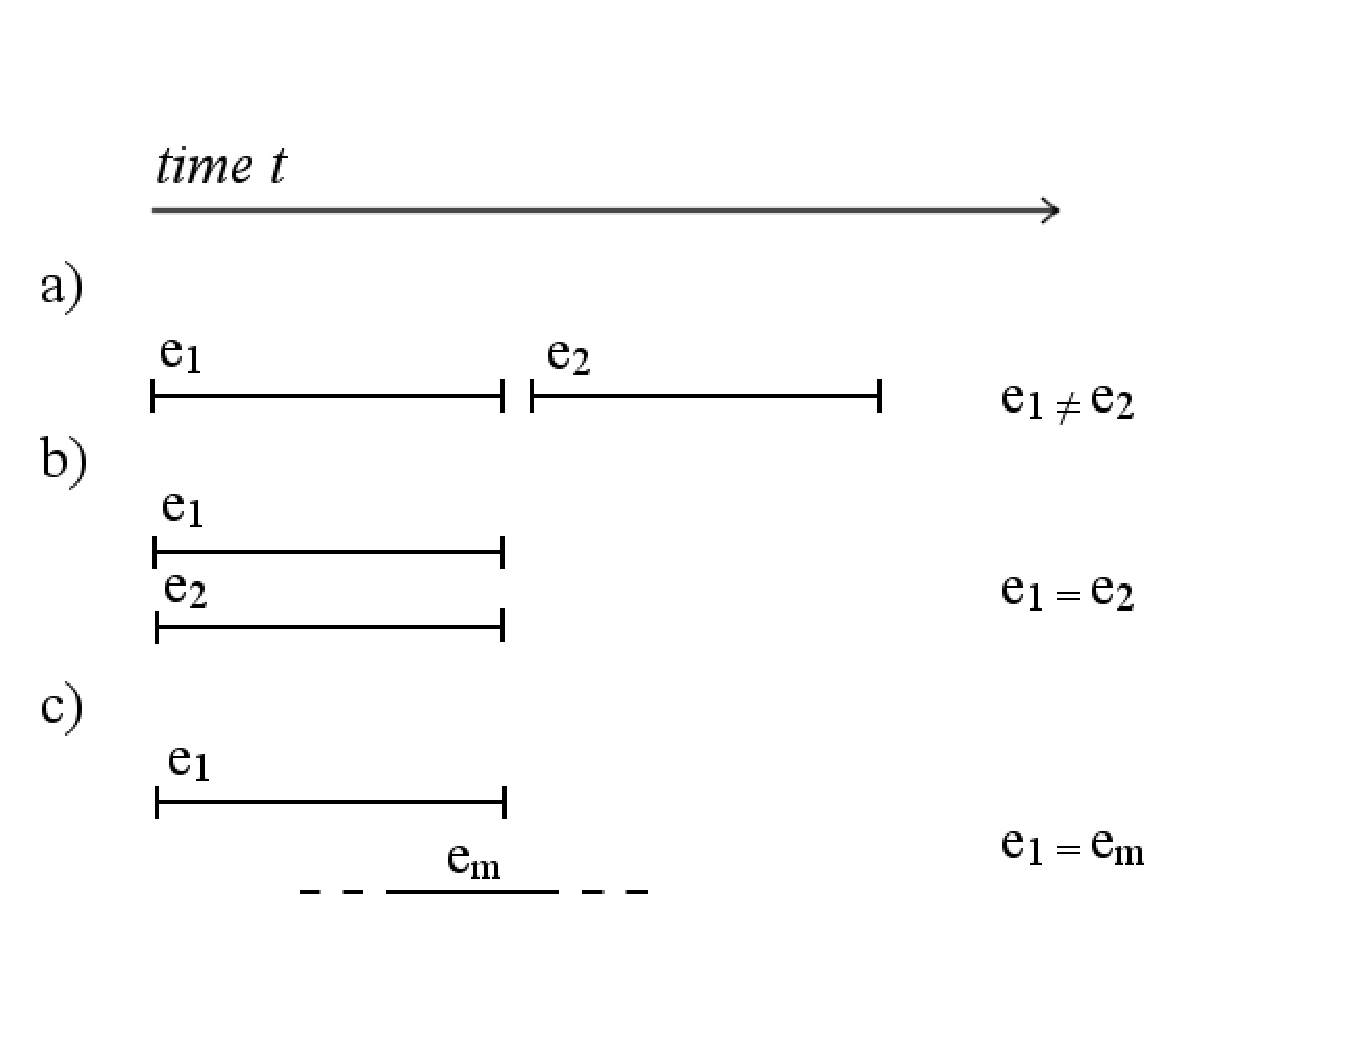
\includegraphics[width=1.0\textwidth]{figures/eventschemav2.eps} 
\caption{Interaction types between event arguments in MVCs}\label{fig:eventsmod}
\end{figure}

At this point, using event arguments does not reveal any explanation as to why the LLEs in type a) do not merge but constitute a staged CLE, while the LLEs in b) do so. But assuming event arguments to be active in the formation of MVCs does provide us with a means to be able to model different temporal configurations.

In the next section, I will have a closer look at lexical decomposition which is particularly helpful when it comes to  merger scenarios as for example \textsc{merging} of motion events in (\ref{WMH_Julio_goat049_2}). Before I close this section, however, I would like to address a further quirk to the event argument analysis. As it turns out, MVCs do not only provide event arguments at the LLE level, they also seem to produce more complex event arguments at higher levels (and thereby arguably confirm the existence of PLEs and CLEs). This becomes clear when MVCs are inserted into Maienborn's event diagnostics listed in (\ref{diagnostics}) above. The first test claims that, as events are perceptible in space and time, linguistic construals of events are permitted to occur as (infinitival) complements in perception verb constructions. If we have a look at the EI area it turns out that this idea is also applicable to MVCs. In Wooi for instance, motion-to-action constructions may occur as complements of perception verbs just like simplex predicates do. Consider the following elicited example (note that the English translation uses an infinitive construction for readability (``accusative and infinitive" in Latin Grammar) -- the original structure in Wooi does not support a raising hierarchy):

\ea \label{hendeho}
\langinfo{Wooi}{Autronesian, SHWNG}{elicit.}
\ea
\glll hende ho kiori ra con ho i \\
he-re ho $<$i$>$ko=i ra ti-ong ho i \\
3\textsc{pl}-eye \textsc{dir} $<$3\textsc{sg}$>$carry=\textsc{obj}.\textsc{sg} go 3\textsc{sg}-give \textsc{dir} 3\textsc{sg}\\
\glft `They saw him carry it there and give it to her.' (lit. they saw him carry go give it to her')\\
\ex
\glll *hende ho i kiori ra con ho i\\
he-re ho i $<$i$>$ko=i ra ti-ong ho i \\
3\textsc{pl}-eye \textsc{dir} 3\textsc{sg} $<$3\textsc{sg}$>$carry=\textsc{obj}.\textsc{sg} go 3\textsc{sg}-give \textsc{dir} 3\textsc{sg}\\
\z
\z

The matrix construction in (\ref{hendeho}) is a nominal predicate consisting of the word for eye and a directional. This is the standard way of encoding visual perception in Wooi. All material that comes after the directional belongs to a (complex) motion-to-action MVC that is subordinated as stimulus argument of \textit{hende ho}. The starred sentence confirms that it is indeed the stimulus argument slot that hosts the MVC: the pronoun \textit{i} can act as a substitute for the action to be perceived, but it cannot co-occur with the full argument spelled out by the MVC. The first sentence, on the other hand, is absolutely fine, as would be \textit{hende ho i} `They saw it'.

Maienborn's second test for hidden event arguments claims that event expressions combine with locative and temporal modifiers. This test accords less well with MVCs from Eastern Indonesia. First and foremost, neither locative nor temporal modifiers typically occur with MVCs which is most probably due to their specific pragmatic function. MVCs tend to be used to sum up paragraph information by repeating the previously introduced verbs in a compressed formula. At the point of the MVC wrap-up, temporal or locative information are usually already known from previous utterances and tend to get dropped during the summarising part. This is why the sample does not contain many examples of MVCs modified with locative or temporal adverbials. If indeed such modifiers co-occur with MVCs the scope is typically confined to one of the stages. Consider the following rather complex MVC from Wooi.

\ea  
\langinfo{Wooi}{Austronesian, SHWNG}{frogstory\_Kosmus}\\
\glll hunda huna husa haherai na wirey \\
hu-ra hu-na hu-ha hahera=i na wirey \\
3\textsc{du}-go 3\textsc{du}-be.at 3\textsc{du}-call search=\textsc{obj}.\textsc{sg} \textsc{loc} forest\\
\glft `Both of them went out into the forest and searched (for the frog).' \\
\z

The whole construction is a motion-to-action MVC at the matrix level, that is, it consists of a precursor motion stage followed by an action stage. Although the forest is by way of inference the goal of the going, the scope of the locative PP \textit{na wirey} at the end is in all likelihood only on the action phase \textit{huna husa haherai} (given the setting in the frogstory, and the specific context of the narration). This illustrates that locative modifiers should provide a good way of testing whether a given MVC is staged (that is, whether it contains two temporal phases) or not. With staged MVCs, the natural scope of the modifier is only on one of the stages, typically the one that is closest to the modifier. Some staged MVCs, however, seem to be ambiguous between two scope interpretations. For instance, resultative MVCs such as the one in example (\ref{keriaviata}) would probably be interpreted as being jointly modified by the locative adverbial, with both stages being inside its scope. But this would need to be tested (for instance with entailment tests), so that I can only suggest such an assumption at this point. Note, however, that such MVCs convey the strong reading of immediate sequence, suggesting that a reading along the lines `die at (unspecified) place x, and remain at place y' would probably be dispreferred, or even impossible.

\ea \label{keriaviata} 
\langinfo{Wooi}{Austronesian, SHWNG}{poison\_for\_animals}\\
\glll keria via na vavaw \\
$<$i$>$karia $<$i$>$va na vavaw \\
$<$3\textsc{sg}$>$die $<$3\textsc{sg}$>$lie \textsc{loc} there\\
\glft `(The animal) will die and remain there.' (lit. `it will die lie there')\\ 
\z

Maienborn's last test, event expressions combining with manner adverbials, comitatives etc, is also possible with MVCs. Construals of motion, for instance, can be targeted by adverbials like \textit{slow} or \textit{fast} (which are usually also regarded as verbs in most of the EI languages). Have a look at the next example from Wooi. Stative verb \textit{mararu} is placed right before a \textsc{motion complex} consisting of the two verbs \textit{vavu} `return.home' and \textit{taveri} `return' (the latter of which does not receive subject indexing in this constructional slot). As both motion verbs contribute facets to the overall motion event, \textit{mararu} targets the whole construction. If modifiers such as \textit{mararu} are argued to operate over a hidden event argument, then it would seem that in (\ref{Wooi41}) the event arguments of both verbs act together. This comes very close to what I called PLE above.

\ea \label{Wooi41} 
\langinfo{Wooi}{Austronesian, SHWNG}{HIVIAY\_exp 077}\\
\glll tamararu tambavu taveri \\
ta-mararu ta-vavu taveri \\
1\textsc{pl}.\textsc{in}-fast 1\textsc{pl}.\textsc{in}-return.home return\\
\glft `We go home fast.' \\ 
\z

What these tests suggest is that MVCs may not only provide LLEs with a hidden event argument but that these event arguments can be bundled and interpreted as one composite event argument, at least with some construction types in some of the languages. The event argument model that I sketched out in Figure \ref{fig:eventsmod} may therefore be extended as in Figure \ref{fig:eventsmod2} in order to capture the range of variation in MVC event construals.

\begin{figure}
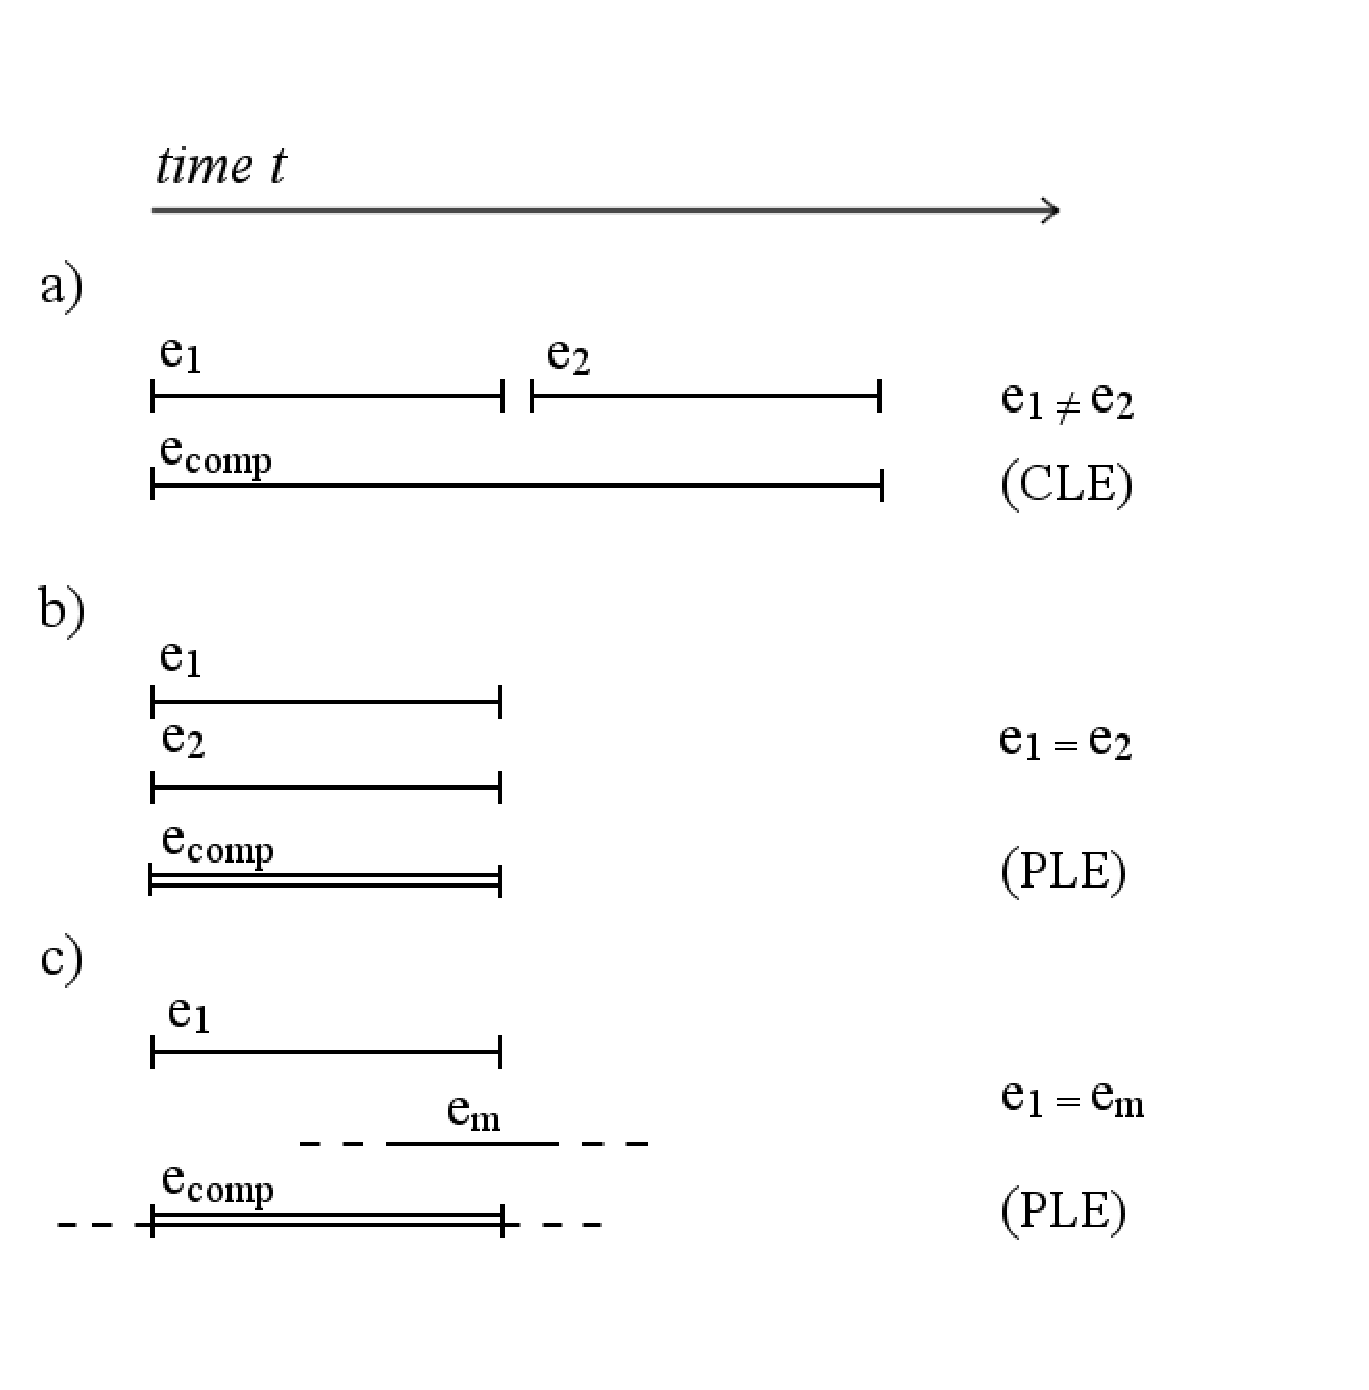
\includegraphics[width=1.0\textwidth]{figures/eventschemamod.eps} 
\caption{Interaction types between event arguments in MVCs, resulting in composite event arguments.}\label{fig:eventsmod2}
\end{figure}


The a) type again is the staged MVC. The event arguments of both verbs are joined together at the clausal level (yielding a CLE), a result that appears also to follow from the fact that the overwhelming majority of such constructions show shared operator scope with grammatical formatives, targeting a composite event schema rather than the underlying LLEs of the verbs. Type b) represents merger MVCs that only consist of one temporal stage. Here, both event arguments can be thought of as being projected on each other (or, to be more precise, $e_2$ fuses with matrix event $e_1$). The resulting composite event (argument) is rooted in the predicate level rather than being aligned with the clausal level (mostly because such construals are allowed to enter stages of higher-level MVCs). The same goes for the modifying type c) where the matrix verb exerts spatiotemporal limits on the modifier thus making its event schema $e_m$ fit into the spatiotemporal frame of $e_1$.

\subsection{Lexical decomposition} \label{sec:decomposition}

It has become clear from the last section that hidden event arguments may motivate different spatiotemporal templates in MVCs, yet they cannot fully explain why staged MVCs do not have their LLEs combined while non-staged MVCs might do so. To this end, this section reviews another semantic approach that might help out in this matter.

Ever since \citet{vendler1957verbs} it has been clear that verbs fall into different event classes. Walking an unspecified distance is different from reaching a summit, or from building a house. This difference in lexical aspect can be demonstrated by applying different grammatical tests, such as using the progressive aspect in English, or adding a temporal frame adverbial such as \textit{for x time} or \textit{in x time}. The different verb classes show different reactions to these tests, thereby justifying the well-known distinction into \textit{states}, \textit{processes} (or \textit{activities}) and \textit{events} (or \textit{transitions}) (see for instance \citealt{pustejovsky1991syntax} for a concise discussion). The latter category denotes eventualities that have a culmination point beyond which a resultant phase occurs with adversative semantics (for instance, the culmination point of \textit{building a house} is the point in time when the house is built). The classical distinction in \citet{vendler1957verbs} is between \textit{achievements} that occur punctually and are typically non-agentive, and \textit{accomplishments} with a durative phase leading up to the culmination point. As opposed to \textit{achievements}, \textit{accomplishments} are volitional actions driven by a willful instigator (building a house would hardly be imaginable without a clear agent).

Another insight from verb class analysis is that one verb may be associated with different verb classes. This is the case with verbs that allow for different argument patterns. If we say that \textit{the door is closed}, we refer to a state of indefinite temporal extension, while \textit{the door closed} would involve a state change between the door being not closed and the door being closed. A construction like \textit{Jones closed the door} would involve a transitive configuration, specifying an actor that causes the state change from $\neg$closed to closed. Another way of changing a verb's class is by adding non-verbal constituents (NPs, PPs, adverbials and so on) to it that alter the event interpretation. An event of \textit{eating apples}, for instance, could go on for quite some time, while \textit{eating an apple} is clearly bound by the size of the apple (and the appetite of the eater). From an event perspective, however, \textit{eating an apple} seems to be quite the same event as, say, \textit{painting a picture}, or \textit{digging up a parsnip}. The central idea with lexical decomposition is to assign a common sublexical structure to all such instances of the ``same" event class in order to explain their identical aspectual behaviour.

According to most contemporary theories of lexical decomposition, the structural part of verb meanings basically consists of a stock of primitive predicates (minimal conceptual events with particular predicate-argument configurations) which license primitive objects (basically things, places etc) to fill their argument positions. Such decomposed meaning primitives are thought to constitute what is called the Lexical-Conceptual Structure (short \textsc{LCS}) of a verbal lexeme. The minimal predicates themselves are allowed to enter argument positions licensed by other primitive predicates according to specific rules of combination (referred to, for instance, as Template Augmentation by \citealt[111]{rappaport1998building}). The claim is that by combining these primitive predicates to more complex predicate-argument structures, a potentially universal set of event types can be established that defines the limits of what event conceptualisations verbs are capable to denote \citep{rappaport1998building, baker2010complex}. A decompositional view on the semantic structure of verbs lends itself particularly well to theories of multi-verb interactions. If semantic structure is confined to and made of a smallish set of minimal predicates then in principle verbs that lexicalize part of the same semantic structure can be expected to merge that structure under certain conditions. This is the line of reasoning that \citet{baker2010complex} adhere to in their application of predicate decomposition to Australian coverb constructions and SVCs from a range of other languages. They argue that there is a fundamental distinction between merger constructions fusing part of their event structure, and coindexing constructions where fusion in a quite different sense pertains to the identity of arguments across different verbs. While this approach is certainly a powerful tool to identify the semantic driving force at work in MVCs, much of its explanative power hinges on the type and amount of primitives that are postulated by decomposition theories.

As \citet{levin2005argument} point out, three basic approaches to semantic decomposition may be distinguished: (i) localist approaches, (ii) aspectual approaches, and (iii) causal approaches. All three of them have focused on specific semantic features (roughly, the semantics of space, time, and reason, or force, respectively) and while all of them have successfully dealt with subsets of verbal predicates, no approach is without shortcomings when it comes to other parts of the verbal lexicon. In what follows I will focus on the localist and aspectual approaches to lexical decomposition, while more or less ignoring the causal approaches (basically because the former two appear to be more suitable to MVC analysis). While both spatial and temporal decomposition are valuable tools with regard to certain verb classes, they are not capable of modelling \textit{all} classes equally well. For instance, localist approaches are great with motion and position verbs but quite bad at motivating the internal structure of, say, verbs of change of possession such as \textsc{take} or \textsc{give}. Therefore, most current takes on verbal decomposition rather make use of a hybrid set of semantic primitives, drawing from ideas from different approaches. In what follows I will give a short account of some of the basic tenets of localist and aspectual approaches, and point out some of their drawbacks when they are applied in a pure fashion. In §\ref{sec:sem-templates}, I will then sketch an approach to model verb classes which is basically informed by what \citet{van1997syntax} present as a semantic decomposition of verb classes within the RRG framwork. I will add some further primitives into the Van Valin and LaPolla system in order to account for the MVC data und the specific behaviour of EI merger constructions.

\subsubsection{Spatial decomposition}

The localist approach claims that the most fundamental cognitive concepts involve the semantic field of motion and location, and that most conceptual semantic structures can be modeled by use of primitives such as \textsc{go}, \textsc{be}, and \textsc{stay}. The localist approach dates back to work by \citet{gruber1965studies}, followed and formally elaborated by \citet{Jackendoff1990}, and has recently been used by \citet{baker2010complex} to motivate their distinction between verbs that undergo predicate merging and other multiverb constructions that involve mere coindexing of shared arguments. The localist approach is particularly good at accounting for all those domains in verb semantics in which a theme is located somewhere or is in motion along a path, including many instances of metaphorical constructions of motion and location in other semantic fiels. Consider the following examples, taken from \citet[25]{Jackendoff1990}:

\ea \label{Jackendoff01} Spatial location and motion
\ea  The bird went from the ground to the tree.
\ex The bird is in the tree.
\ex Harry kept the bird in the cage.
\z
\z

\ea \label{Jackendoff02} Possession
\ea The inheritance went to Philip.
\ex The money is Philip's.
\ex Susan kept the money.
\z
\z

\ea \label{Jackendoff03} Ascription of properties
\ea The light went/changed from green to red. \\
Harry went from elated to depressed.
\ex The light is red. \\
Harry is depressed.
\ex Sam kept the crowd happy.
\z
\z

While the examples in (\ref{Jackendoff01}) illustrate basic construals of motion and location, other semantic fields as well show similar ways of construal. Take for instance the semantic field of possession illustrated in (\ref{Jackendoff02}): possessed referents can be `moved' from one participant to another, adessive construals of possessor and possessee are a typologically frequent way of expressing alienable possession, and so on. The same metaphorical connection to construals of motion and location holds for many other semantic fields and is proposed to inherently underly such predicate classes as change of state predicates, states, and predicates of prolonged engagement (cp. (\ref{Jackendoff03})), demonstrating the pervasive role scenarios of motion and location play in human cognition. According to the Thematic Relations Hypothesis (\citealt{gruber1965studies}, adapted in \citealt{Jackendoff1990}), both the basic construals of motion and locations as well as the derived ones are claimed to be realisations of the same underlying conceptual functions, illustrated in (\ref{themrel}) \citep[26]{Jackendoff1990}.

\ea \label{themrel}
Basic conceptual functions of motion and location
\z

\avmsortfont{\itshape}
{\scriptsize
\begin{avm}
\sort{Event}{\[
GO 
\( \[ \hspace{20pt} \], \sort{Path}{\[ 
FROM \(\[ \hspace{20pt} \]\) \\
TO \(\[ \hspace{20pt} \]\) \]} 
\) 
\]}
\end{avm}
}

\smallskip
{\scriptsize
\begin{avm}
\sort{State}{\[
BE 
\( \[ \hspace{20pt} \], \sort{Place}{\[ \hspace{20pt} \]} 
\) 
\]}
\end{avm}
}

\smallskip
{\scriptsize
\begin{avm}
\sort{Event}{\[
STAY 
\( \[ \hspace{20pt} \], \sort{Place}{\[ \hspace{20pt} \]} 
\) 
\]}
\end{avm}
}

\bigskip
The conceptual function \textsc{go} has two arguments, a theme argument denoting the entity under motion, and a path argument which in turn may host a set of monovalent path predicates, such as \textsc{from}, \textsc{to}, or \textsc{via}. The two location functions \textsc{be} and \textsc{stay} also denote a theme argument combined with a place. As many verbs appear in constructions that involve motion and/or location subevents, these conceptual functions are frequently used in modelling more complex event structures. To illustrate, take for instance the event semantics of \textsc{putting} some object at some place, apparently including a motion component (the theme that is relocated) and a goal component (the place at which the theme is put to rest). Quite intuitively, the event template of a \textsc{put} predicate would invite the use of the conceptual functions \textsc{go} (or \textsc{move}) and \textsc{be} in order to capture these semantic components. Baker and Harvey propose the following conceptual structure for the merger construction (\ref{Marra03}) in the Australian language Marra, consisting of the coverb \textit{birli} `go in' and the light verb \textit{ganji} `take' \citep[24f.]{baker2010complex}. The merging results in a combined stucture \textit{birli ganji} which means `put in':

\ea \label{Marra01}
\textit{birli} `go in': {\small[$_{Event}$ MOVE ([$_{Thing}$ x ], [$_{Path}$ IN ])]}
\z
\ea \label{Marra02}
\textit{ganji} `take': {\small[$_{Event}$ CAUSE ([$_{Thing}$ y ], [$_{Event}$ MOVE ([$_{Thing}$ x ], [$_{Path}$ ])])]}
\z

\ea \label{Marra03}
\textit{birli + ganji} `put in': \\
{\small[$_{Event}$ CAUSE ([$_{Thing}$ y ], [$_{Event}$ MOVE ([$_{Thing}$ x ], [$_{Path}$ IN ])])]}
\z

By combining the event templates of \textit{birli} in (\ref{Marra01}) and \textit{ganji} in (\ref{Marra02}) to the joint conceptual structure of \textit{birli ganji} in (\ref{Marra03}), the functions \textsc{cause} and \textsc{move} enable the theme argument x to be transferred by the causing referent y along a path \textsc{in} to a place inside a container, where \textsc{in} is shorthand for a more complex path-goal combination like [\textsc{to} [\textsc{in} $<$place$>$]] (see \citealt[45]{Jackendoff1990}). The light verb \textit{ganji} provides the structural skeleton of a three participant event construal (causer, theme, and path), while the coverb \textit{birli} contributes specific content on the motion path traversed by the theme. 

Evidently, the use of \textsc{go} (or \textsc{move}, for that matter\footnote{In the following discussion and throughout the book, I regard \textsc{go} and \textsc{move} essentially as synonymous notations for a predicate function that involves physical motion or movement and licenses a path argument (see also \citealt[27]{baker2010complex} for a similar stance).}) seems felicitous iff a verb has among its options of argument expression construals in which it combines with path modifiers, such as \textsc{put} allows in English (as in \textit{Jones put the toast on the table}). However, the claim of the Localist Approach extends beyond verb semantics of physical orientation and seeks to account for many other verb classes where physical motion figures less prominently or may even be absent. This is in particular the case with certain classes of activity verbs and change-of-state verbs where a \textsc{move} component would make wrong predictions with regard to predicate merging. I will illustrate the problem of \textsc{move} generalization with the case of change-of-state verbs. For example, in their discussion of merger constructions in Wagiman (Australian) Baker and Harvey provide the following LCS for \textit{du} `cut':

\ea \label{Wagiman01}
\textit{du} `cut': \\
{\small[$_{Event}$ CAUSE ([$_{Thing}$ ], [$_{Event}$ MOVE ([$_{Thing}$ ], 
[$_{Path}$ TO ([$_{Place}$ IN [$_{Thing}$ ]])])])]}
\z

The transitive argument configuration is modeled by a \textsc{cause} predicate licensing an actor argument, and an embedded \textsc{move} predicate that is further subcategorized for an object and a path function referring to the goal argument of the cutting. The reason for assuming such a LCS is probably that from a spatiotemporal point of conception, the postulation of a path trajectory for an instrument (such as a knife or other object with a sharp blade) dissecting a patient argument makes perfect sense. There is, however, room for doubt whether this trajectorial part is really lexicalized in \textsc{cut} verbs in this way. In particular, two objections may be raised. First, though not commented on directly by Baker and Harvey, the first argument of the \textsc{move} function can only be logically understood as the instrument of cutting. As argument slots licensed by predicate functions ought to map on morphosyntactic arguments, we would expect that the instrument as such is realised as a subcategorised argument rather than an instrument adjunct. That is, at least one of the event templates \textsc{cut} occurs with should display an instrument phrase in object function combined with a path argument. One way to put the semantic structure to a test is to look at the licit patterns of argument realisation of \textsc{cut} verbs. Starting with the work of \citet{Fillmore1970}, verb classes in English and other languages have often been analysed and argued for by virtue of comparing so-called diathesis alternations, specific alternations in the morphosyntactic expression of arguments, which verbs of the same verb class participate in \citep{Levin1993}. Verbs of \textsc{hitting}, \textsc{breaking}, and \textsc{cutting} have received major attention because these verb classes differ in specific ways by permitting specific subsets of these alternations. Consider the following examples (taken from \citealt[148f. and 156]{Levin1993}):

\ea Basic transitive argument realisation \label{alt01}
\ea Carol hit the fence
\ex Carol cut the bread
\z
\z

\ea Instrument Subject Alternation \label{alt02}
\ea Carol hit the fence with a stick
\ex Carol hit the fence
\ex Carol cut the bread with a knife
\ex Carol cut the bread
\z
\z

\ea Middle Alternation \label{alt03}
\ea[*]{The fence hits easily}
\ex[]{Paula hit the fence}
\ex[]{Whole wheat bread cuts easily}
\ex[]{Carol cut the whole wheat bread}
\z
\z

\ea With/Against Alternation \label{alt04}
\ea[]{Carol hit the stick against/on the fence}
\ex[]{Carol hit the fence with the stick}
\ex[*]{Carol cut the knife against/on the bread}
\ex[]{Carol cut the bread with the knife}
\z
\z

The basic transitive construction in (\ref{alt01}) is fine with both the \textsc{hit} and the \textsc{cut} class, and so is the Instrument Subject Alternation in (\ref{alt02}) where an instrument adjunct is added. The alternations given in (\ref{alt03}) and (\ref{alt04}), however, are only applicable to one of the two classes: while \textsc{cutting} allows the Middle Alternation in which the patient argument is promoted to subject function, the \textsc{hitting} class does not. The reverse is true for the With/Against Alternation where the instrument argument is promoted to direct object function and the patient argument is realised as oblique. It is particularly this alternation that is interesting in the light of the predicate decomposition of Wagiman \textit{du} `cut' above: as the alternation shows, \textsc{hit} verbs do lexicalise an instrument-path template in which the instrument is moved along a path on a patient argument. Therefore, \textsc{hit} verbs may well receive the same predicate decomposition as for instance relocation verbs such as `put' in (\ref{Marra03}) above. \textsc{cut} verbs, on the other hand, do not seem to offer such an instrument-path template and are therefore probably better analysed as change-of-state verbs involving an activity or accomplishment decomposition by making use of a [CAUSE [BECOME [BE]]] combination.

The second objection that may be raised against a localist decomposition of \textsc{cut} verbs directly pertains to  predictions of predicate merging that would follow from a \textsc{move} component. In my Eastern Indonesian sample, several transitive verb classes are attested that are open to verbal path modification provided by a motion verb in V$_2$ position. According to the glosses used in the data, \textsc{hit} verbs, \textsc{take} verbs, object relocation verbs such as \textsc{put} or \textsc{pour}, verbs of force exertion (\textsc{pulling} and \textsc{pushing}), and other transitive verbs like verbs of directed sensual perception may be modified in such a way (possibly with different languages allowing different verb classes to undergo verbal path modification). \textsc{cut} verbs, however, are not among them, which suggests that they function differently from verbs that directly lexicalise path components as basic part of their meaning.

Therefore, I conclude that a cogent analysis using predicate decomposition to motivate the formation of certain kinds of multi-verb constructions would need to base the semantic templates on the morphosyntactic behaviour of the constructions attested in the sample. Localist predicate decomposition develops a particularly strong explanative force with those construals in which the patterns of argument realisation closely mirror the proposed underlying predicate semantics. The use of \textsc{move} predicates, however, should be limited to those verbs that either lexicalise a translational motion event or else a movement path pertaining to object relocation (thematic relation), object affection (patientive relation), or directed sensation.
It would seem logical that for those instances in which motion is indeed a valid function to occur in semantic structure, the inference should hold that at the final event boundary, the moving object should have reached its designated place. We may formalise this inference by using Jackendoff's inference rule given in (\ref{Jackendoff04}) and limit its scope to instances of motion proper \citep[27]{Jackendoff1990}:

\ea \label{Jackendoff04} Inference rule \\
At the termination of [$_{\textit{Event}}$ GO ([X], [$_{\textit{Path}}$ TO ([Y])])], \\
it is the case that [$_{\textit{State}}$ BE ([X], [$_{\textit{Place}}$ AT ([Y])])].
\z

Thus, strictly speaking, if Jones cuts a bread into slices it is not the case that either Jones or the bread partake in a motion event (and the knife as a moving instrument should be ruled out from filling the argument position [X] on the basis of the evidence from diathesis alternations sketched above). This is not to say that motion is totally absent from the event conceptualisation of cutting. Most if not all dynamic events may involve motion conceptualisations of some sort. Yet, I think that it is only with certain verb classes that motion as a templatic feature takes centerstage in event lexicalisation.

\subsubsection{Aspectual decomposition}

Another approach to predicate decomposition is rooted in theories of aspectual verb classes. The aspectual approach starts out from the by now classical observations into lexical aspect initiated by Vendler's work on verb classes in English: the differentiation of states, acitivites, achievements, and accomplishments basically revolves around the notions of stativity, punctuality, and telicity with statives being different from the other three classes by virtue of being stative (or non-dynamic), activities by having no inherent endpoint (being atelic), and achievements by being telic but punctual (without temporal duration) as opposed to accomplishments (see e.g. \citealt{levin2005argument, croft2012verbs}). A typical feature space of the Vendler classes is given in Table \ref{table:Vendler} (taken from \citealt[93]{van1997syntax}).

\begin{table}
\begin{tabular}{lccc}
\lsptoprule
\multicolumn{1}{l}{class}&\multicolumn{1}{c}{static}&\multicolumn{1}{c}{telic}&\multicolumn{1}{c}{punctual}\tabularnewline
\midrule
State&+&\textminus&\textminus\tabularnewline
Activity&\textminus&\textminus&\textminus\tabularnewline
Accomplishment&\textminus&+&\textminus\tabularnewline
Achievement&\textminus&+&+\tabularnewline
\lspbottomrule
\end{tabular}
\caption[Feature combination of Vendler verb classes]{Feature combination of Vendler verb classes (from \citealt[93]{van1997syntax})}
\label{table:Vendler}
\end{table}

The most important evidence for the feature combinations shown in Table \ref{table:Vendler} comes from insertion tests, starting with Vendler's seminal study \citep{vendler1957verbs}. Each feature is tested by constructing a carrier frame or by applying a grammatical category to the verb: the stative/dynamic distinction can be shown by applying the English progressive which is acceptable for dynamic verbs but not for statives. For example, while \textit{I am running} is a well-formed answer to the carrier question \textit{What are you doing?}, \textit{*I am knowing it} is definitely not \citep[35]{croft2012verbs}. The punctual/durative distinction can be tested by applying temporal question pairs such as \textit{At what moment...?} vs \textit{For how long...?}. Achievement verbs like \textit{spot} only license a punctual time frame (cp. \textit{At what moment did you spot the plane?} and \textit{*For how long did you spot the plane?}, op.cit.) in contrast to the other verb classes which are prototypically construed with a durative time frame (but see \citealt{croft2012verbs} for alternative construals). Finally, the atelic/telic or unbounded/bounded distinction becomes apparent when temporal adverbials are added: with durative temporal adverbials such as \textit{for ... [time]} in English, no natural endpoint is implied and the event may end without having reached a state change. Thus, construals of activity verbs as in \textit{He pushed the cart for half an hour} are fine, while construals with accomplishment verbs as in \textit{?She drew the circle for half an hour} seem odd (yet here again, alternative construals are available for some verbs). Construals involving the container adverbial \textit{in ... [time]} just show the reverse pattern. While they readily modify bounded/telic verbs (cp. \textit{She drew the circle in twenty seconds}), construals of activity verbs are generally rejected (with the exception of activity verbs that allow for an accomplishment construal, such as \textit{*Erin ate in two minutes} vs \textit{Erin ate the apple in two minutes}, see \citealt[99]{van1997syntax} and \citealt[38]{croft2012verbs}). In more recent work on lexical aspect, more fine-grained class distinctions have been proposed yet the original four Vendler classes still constitute the backbone of most aspectual approaches to verb semantics. \citet{croft2012verbs} provides a comprehensive overview of the different subclasses and additions proposed in the literature.

Aspectual approaches to verb decomposition take the idea of aspectual verb classes as a vantage point for deconstructing verbal semantics. The conceptual primitives that are used to model the aspectual classes include \textsc{be} for stative verbs, \textsc{do/act} for activity verbs, and \textsc{become} (and \textsc{ingr}(essive) in Van Valin and LaPolla's RRG framework) for bound verbs (achievements and accomplishments). Unlike in the localist approach, the notions of motion and position are not granted the status of independent semantic functions in aspectual frameworks but are subsumed as subsets under different aspectual classes. This has some advantages and at the same time poses certain difficulties. For instance, \citet[106]{van1997syntax} point out that motion path verbs like \textsc{come} and \textsc{go}, contained motion verbs like \textsc{enter}, and motion ground verbs such as \textsc{arrive} may conceptualise either punctual or durative events in different languages. This variation in temporal extension is probably better captured within an aspectual verb class model where the class distinctions directly reflect the temporal properties of the event conceptualisations. To illustrate the point, manner of motion verbs can be construed both as atelic activity verbs and as telic accomplishments depending on the arguments realised in the clause. One solution to this variation is to make use of semantic functions that directly pertain to the aspectual type of event. Consider the following examples from \citet[111]{van1997syntax}:

\ea \label{VanValin:run}
\ea Paul ran. \label{VanValin:runa}
\exi{a'} \textbf{do'} (Paul, [\textbf{run'} (Paul)])
\ex Paul ran to the store. \label{VanValin:runb}
\exi{b'} \textbf{do'} (Paul, [\textbf{run'} (Paul)]) \& \textsc{become} \textbf{be-at'} (store, Paul)
\z
\z

In example (\ref{VanValin:runa}) the event of running is construed as an unbound activity since no argument is realised that would impose a temporal boundary on the event. The atelic activity reading is directly reflected by use of the empty activity predicate \textbf{do'}. In example (\ref{VanValin:runb}), on the other hand, the running event is temporally delimited to the distance from the starting point up to the place of the store. The telic reading of this predicate is accounted for by adding an accomplishment predicate to the activity, connected through the predicate connective `\&'. The advantage here is obvious: running in its activity reading directly classes with other activity predicates like \textsc{eat}, \textsc{sweep}, \textsc{talk} and so on. By contrast, localist approaches cannot deal with activity verbs in such a straightforward way. To give just two examples, consider the semantic templates for \textsc{walk} (\ref{Baker:walk}) and \textsc{eat} (\ref{Baker:eat}) as proposed by \citet{baker2010complex}:\footnote{For sake of convenience, I adopt a simplified notation of Jackendoff's, and Baker and Harvey's framework from now on. Specifically, I only make use of the square brackets [ ] in cases where they increase the overall readability of the formula, i.e., when an argument itself contains a predicate with a set of subcategorized arguments. Also, I don't give subscribed labels such as \textit{event}, \textit{thing}, or \textit{place} as they are mostly inferable from the structural position.}

\ea \label{Baker}
\ea \textsc{move} (x, \textsc{path}) \label{Baker:walk}
\ex \textsc{cause} (x, [\textsc{move} (y, \textsc{path})]) \label{Baker:eat}
\z
\z

Baker \& Harvey propose a generic \textsc{move} predicate to account for activity predicates, roughly following Jackendoff's  localist analysis (though conflating \textsc{move}(x) and \textsc{go}(x,\textsc{path}) into a single primitive \textsc{move}). Intransitive activity predicates generally follow the schema depicted in (\ref{Baker:walk}). The subscribed semantic content of the verb complements the generic function \textsc{move}, realised with a subject referent x and optionally a path component. Transitive activity verbs, such as \textsc{eat}, however, are rendered in a different manner in order to capture the difference in argument frame (actor plus patient argument). Here, the actor argument is licensed by the predicate \textsc{cause} which as a second argument takes the activity configuration \textsc{move}(y,\textsc{path}). The latter, however, can hardly be thought of as constituting an independent activity predicate as it might be expected from a comparison with, say, break verbs that allow for the causative alternation, cp. \textit{The thief broke the window} vs. \textit{The window broke}. There is no such alternation for \textsc{eat} in English that would provide evidence for an analysis along the lines of (\ref{Baker:eat}). While the Unspecified Object Alternation is fine (\textit{Cynthia ate the peach} vs. \textit{Cynthia ate}; \citealt[213]{Levin1993}) no such alternation is possible between a transitive argument realisation (\textit{Cynthia ate bread}) and an intransitive one with the patient being promoted to subject position (\textit{*The bread eats}).\footnote{The middle alternation, on the other hand, seems licit in certain contexts, for example \textit{This bread eats like a meal} (Google search). Using a \textsc{cause} function to model transitive activity/accomplishment predicates is also problematic for another reason as analytical causatives like \textit{Peter made Cynthia eat the bread} would derive a predicate structure with two instances of causing, Peter causing Cynthia to eat, and Cynthia causing the bread to move. That extensive use of \textsc{cause} in lexical decomposition would give rise to problems of that kind has also been noted by \citet{Jackendoff1990}.} In aspectual approaches like \citet{rappaport1998building} or \citet{van1997syntax} the challenge posed by transitivity contrasts is deferred to the semantic content. Compare the examples in (\ref{VanValin:drink}) from \citet[111]{van1997syntax}:

\ea \label{VanValin:drink}
\ea Carl drank beer. \label{VanValin:drinka}
\exi{a'} \textbf{do'}(Carl, [\textbf{drink'}(Carl, beer)])
\ex Carl drank a beer. \label{VanValin:drinkb}
\exi{b'} \textbf{do'}(Carl, [\textbf{drink'}(Carl, beer)]) \& \textsc{become} \textbf{consumed'}(beer)
\z
\z

Instead of introducing an internal \textsc{cause} function (as opposed to external \textsc{cause} functions as in \textit{Floyd made Carl drink the beer}) to the semantic template, the transitive argument configuration of the drinking event in (\ref{VanValin:drinka}) and (\ref{VanValin:drinkb}) is reflected by the way the activity class is built: the empty activity predicate \textbf{do'} takes as arguments both an actor and an action. This action slot is filled with the original semantic content of the predicate in question (here \textbf{drink'}(x,y)), displaying either an intransitive or a transitive subcategorization frame. Modelling transitive activity predicates this way retains a unique activity template and confirms the identical behaviour of activity verbs that is evidenced by the Vendler tests (\textit{What are you doing? I am running/I am drinking beer}). 

A further advantage of Van Valin and LaPolla's system is that by addition of a change-of-state predicate the distinction in aspectual construal between activity and accomplishment readings in (\ref{VanValin:drink}) comes out most clearly. At the same time, however, this practice of suffixing additional semantic functions has some untoward effects on the arrangement as well as the interpretation of the logical structure of predicates. First, any addition to the structure might conflict with the assumption that any material in the event structure should match with syntactic constituents. For example, in terms of well-formedness conditions on the syntactic realisation of event structures, \citet[112]{rappaport1998building} propose the Subevent Identification Condition:
 
\ea \textbf{Subevent Identification Condition:} Each subevent in the event structure must be identified by a lexical head (e.g., a V, an A, or a P) in the syntax 
\z

If we apply this condition to example (\ref{VanValin:drinkb}) above, it is not immediately clear which part of the syntactic structure would identify the change-of-state subevent \textsc{become} \textbf{consumed'} (beer). The only structural difference between (\ref{VanValin:drinka}) and (\ref{VanValin:drinkb}) is the use of the indefinite article but even if we assume a DP with the determiner acting as its head (the general rule would then be something like: any countable (number of) object(s) would turn an activity predicate into an accomplishment predicate) the question would remain how \emph{activity} readings with a specified object referent could be dealt with (for instance, with progressives: \textit{Carl was drawing a circle}/\textit{Carl was drawing a circle for ten seconds when suddenly Cynthia distracted him}). 

A second unwanted effect appears with motion predicates that take a path argument. If we have another look at example (\ref{VanValin:runb}) above (repeated below as (\ref{VanValin:runbrep})), we recognise that the path semantics again is supplied by addition of a change-of-state event \textsc{become}. 

\ea \label{VanValin:runbrep}
\ea Paul ran to the store. 
\ex \textbf{do'}(Paul, [\textbf{run'}(Paul)]) \& \textsc{become} \textbf{be-at'}(store, Paul)
\z
\z

This is fine as long as the path is understood as being fully traversed to its end. However, it becomes problematic when the path only encodes a \emph{direction} of the motion (for instance, when the theme moves \textit{towards} some destination without necessarily reaching it). This is the situation that \citet[569]{dowty1991thematic} has discussed under the label \textsc{holistic theme} where it is not part of \textit{Paul} that changes during the runtime of the event but part of the path \textit{to the store} that is traversed. If the semantic content itself, i.e., the motion predicate, wouldn't license a path argument in and of itself where do we get it from if the path is not fully traversed (that is, no state change \textsc{become} \textbf{be-at'} is actually reached)?  Compare the following examples from English and German:

\ea
\ea Paul ran to the store.\label{runstorea}
\ex Paul was running to the store when he realised that he had forgotten his wallet.\label{runstoreb}
\z
\z

\ea 
\ea \label{runstoreag}
\gll Paul rannte zum Laden\\
Paul run:\textsc{3}\textsc{sg}.\textsc{pst} to.\textsc{def} shop \\
\glft `Paul ran to the store.'\\
\ex \label{runstorebg}
\gll Paul rannte zum Laden, aber er kam dort nicht an.\\
Paul run:\textsc{3}\textsc{sg}.\textsc{pst} to.\textsc{def} shop but he arrive:\textsc{3}\textsc{sg}.\textsc{pst} there not \textsc{ptl} \\
\glft `Paul ran to the store but he did not arrive there.'\\
\z
\z

In (\ref{runstorea}) and (\ref{runstoreag}), the path argument creates an accomplishment reading by default and it is assumed that Paul finally got there. In (\ref{runstoreb}) and (\ref{runstorebg}), however, the reading of the path argument is atelic and the full path is not necessarily traversed by the actor/theme. In the English example, it is the choice of the progressive aspect that neutralizes or backgrounds the telicity typically brought about by path arguments. Therefore, we may add a temporal clause stating that in the process of traversing the path to the store something else happened and that this may have led Paul to abort his action. In German, the accomplishment reading may even be disabled within the same tense without employing any overt aspect operator. The crucial point here is that by encoding the path argument of certain predicates as an additional change-of-state function complications arise that could be avoided if the path argument would be licensed directly in the semantic structure of the predicate, as is done in localist approaches to predicate decomposition.

In the light of the EI data that I will present below, the best solution would be to assume that path specifications to motion or movement events are directly encoded within the semantic structure of the verb. At the same time it would be detrimental to assume \textsc{move}, \textsc{stay} or \textsc{be} components for all predicate classes as this would basically allow the merging of motion components between almost all predicates and thus would strongly reduce the predictive power of any component-matching model. However, the EI data clearly suggest that merging of semantic structure only occurs between certain verb classes.

Wrapping up the discussion so far, we have seen that localist and aspectual approaches to lexical decomposition both have qualities that make them the best choice with certain verb classes. Localist approaches perform particularly well with verbs permitting path expressions and locative arguments. Aspectual approaches, on the other hand, gain from their ability to directly account for differences in the temporal coding of events and perform better with the original Vendler classes such as activities, or change-of-state predicates. Given that each approach has its own strength, most current frameworks actually combine functions of both strands, forming mixed approaches to lexical decomposition. The next section presents an outline of such a hybrid approach. It is mostly based on Van Valin and LaPolla's system yet includes also some further variables and subclasses that will allow modelling of MVC behaviour in the EI area, as I will show in the subsequent sections.

\subsubsection{Semantic templates in MVC analysis} \label{sec:sem-templates}

In the preceding section, discussion of the path semantics in examples like (\ref{runstoreb}) or (\ref{runstorebg}) revealed that it seems preferential for certain verb classes to include an inherent option for a path expression into their LCS. I proposed that there are verb classes in which a general ability of licensing path projections is entrenched somewhere in their lexical representation. In the present section, I will suggest a way in which the insights from localist approaches, i.e. assuming path arguments to be part of a LCS, can be combined with a decomposition model that is based on aspectual verb classes. To this end, I will basically use the notational system of \citet{van1997syntax} and add to it additional empty predicate functions in order to model the possible fusion scenarios between different classes of EI verbs. I will show that these structural predicates accord with some of the subclasses associated in \citet{van1997syntax} with specific sets of thematic relations. Table \ref{table:semtemp} gives a list of the different semantic templates assumed by Van Valin and LaPolla, complemented with additional predicate functions that I assume in order to account for the MVC merging scenarios.

\begin{table}
\begin{tabular}{ll}
\lsptoprule
\multicolumn{1}{l}{Verb class}&\multicolumn{1}{l}{Semantic template}\tabularnewline
\midrule
State&\textbf{pred'} (x) or (x,y)\tabularnewline\tabularnewline
Activity&\textbf{do'} (x, \textbf{pred'} (x) or (x,y))\tabularnewline
Motion activity&\textbf{do'} (x, \textbf{move'} (x, \textsc{path}, \textbf{pred'} (x) or (x,y)))\tabularnewline
Speech activity&\textbf{do'} (x, \textbf{say'} (x, \textsc{scont}, \textbf{pred'} (x)))\tabularnewline\tabularnewline
Achievement&\textsc{ingr} \textbf{pred'} (x) or (x,y) or\tabularnewline
&\textsc{ingr} \textbf{do'} (x, \textbf{pred'} (x) or (x,y))\tabularnewline\tabularnewline
Accomplishment&\textsc{become} \textbf{pred'} (x) or (x,y)\tabularnewline
&\textsc{become} \textbf{do'} (x, \textbf{pred'} (x) or (x,y))\tabularnewline\tabularnewline
Causative&$\alpha$ \textsc{cause} $\beta$ where $\alpha$, $\beta$ are LSs of any type\tabularnewline
\lspbottomrule
\end{tabular}
\caption[Semantic templates of verb classes, adapted from \citet{van1997syntax}]{Semantic templates of verb classes, adapted from Van Valin \& LaPolla's lexical representations for Aktionsart classes \citep[109]{van1997syntax}. The predicates \textbf{move'} and \textbf{say'} have been added in order to model motion and speech activity subclasses, respectively.}
\label{table:semtemp}
\end{table}

Van Valin and LaPolla's lexical representations consist of two basic components: constants and variables. Constants are given in boldface and are marked by a prime. Variables are printed in normal typeface. Each constant symbolises a predicate and is associated with a set of arguments. States and activities are understood as the most basic verb classes. States are represented by a single \textbf{pred'} function, activities are composed of an empty activity predicate \textbf{do'} that takes two arguments: the x argument denotes the effector of the activity (where effector stands for any role within the set of actor-like roles that are licensed by activity verbs), and another argument slot that is filled by the actual predicate constant \textbf{pred'}. The empty activity predicate \textbf{do'} basically acts as the marker of membership in the aspectual class of activites and submits additional information on the thematic role of the first argument x (see \citealt[103f.]{van1997syntax} for reasons to assume an empty \textbf{do'}). Note that the two \textbf{pred'} constants in states and activities are not meant to designate the \emph{same} set of predicates. Rather, the members of the activity \textbf{pred'} typically exclusively occur with \textbf{do'} \citep[103]{van1997syntax}. States and activities are thus mutually exclusive inasmuch as that neither can be derived from the other.\footnote{There are, however, exceptions to this in Van Valin and LaPolla's analysis, for instance in their treatment of perception verbs. While seeing is treated as a two-place state, looking is proposed to possess a derived structure containing the same \textbf{pred'}. Consider example (\ref{look}) from \citet[121]{van1997syntax} where the perception state is inserted into an activity LS.

\ea \label{look}
\ea Tanisha looked at the comet with a telescope.
\ex \textbf{do'} (Tanisha, [\textbf{see'} (Tanisha, comet) $\wedge$ \textbf{use'} (Tanisha, telescope)])
\z\z

}

This is why states and activities are analysed as basic verb classes whereas achievements, accomplisments and causative predicates are secondary classes: they either take states or activities as their base. The derivation process of achievements and accomplishments is represented in Van Valin and LaPolla's system by addition of a semantic modifier. Both modifiers take as input a state or activity predicate and derive a telic predicate structure: \textsc{ingr}(essive) marks a punctual change as is commonly associated with Vendlerian achievements, and \textsc{become} denotes a phasic change in which a state change is gradually achieved over time. Examples for each verb class are given below (taken from \citealt[105]{van1997syntax}):

\ea
\ea \textit{States} \\
\begin{tabular}{ll}
The window is shattered.&\textbf{shattered'} (window)\tabularnewline
Fred is at the house.&\textbf{be-at'} (house,Fred)\tabularnewline
John saw the picture.&\textbf{see'} (John,picture)\tabularnewline
\end{tabular}
\ex \textit{Activities} \\
\begin{tabular}{ll}
The children cried.&\textbf{do'} (children, [\textbf{cry'} (children)])\tabularnewline
The wheel squeaks.&\textbf{do'} (wheel, [\textbf{squeak'} (wheel)])\tabularnewline
John ate fish.&\textbf{do'} (John, [\textbf{eat'} (John,fish)])\tabularnewline
\end{tabular}
\ex \textit{Achievements} \\
\begin{tabular}{ll}
The window shattered.&\textsc{ingr} \textbf{shattered'} (window)\tabularnewline
The balloon popped.&\textsc{ingr} \textbf{popped'} (balloon)\tabularnewline
John glimpsed the picture.&\textsc{ingr} \textbf{see'} (John,picture)\tabularnewline
\end{tabular}
\ex \textit{Accomplishments} \\
\begin{tabular}{ll}
The snow melted.&\textsc{become} \textbf{melted'} (snow)\tabularnewline
The sky reddened.&\textsc{become} \textbf{red'} (sky)\tabularnewline
Mary learned French.&\textsc{become} \textbf{know'} (Mary,French)\tabularnewline
\end{tabular}
\z
\z


The examples above illustrate the idea that states (and activities) are the base components in derived LSs: the two-place stative predicate \textbf{see'}, for instance, can be turned into a punctual state-change predicate by adding the modifier \textsc{ingr}. In contrast to the empty activity predicate \textbf{do'}, the semantic modifiers \textsc{ingr} and \textsc{become} do not have an argument frame and do not introduce thematic roles so that the thematic role of, say, the sky in the accomplishment example \textit{The sky reddened} is the same as in the underlying stative base form. Empty \textbf{do'}, however, does impose a thematic role on its predicate constant: we know that the children are not only licensed as argument by the predicate \textbf{cry'} but that \textbf{do'} entails that the children in fact effect the whole event (which is arguably not the case for the sky or the balloon, and not necessarily so for John or Mary in the examples above). Yet we can say that the wheel effects the squeaking, and John effects the event of eating fish. In order to decompose verbs into the basic Vendler classes, it is sufficient in the system of Van Valin and LaPolla to assume three devices (empty \textbf{do'} and the two semantic modifiers) that would turn predicate constants into the four classes. It becomes clear from the few examples, however, that these broad classes fall into a range of subclasses with regard to the thematic relations that are expressed by the first (and second) argument. Within the class of activity verbs, the first argument not only denotes a rather unspecific thematic relation \textsc{effector} but may be subclassified on a more fine-grained scale: with motion verbs, for instance, the \textsc{effector} is the moving entity, i.e., the first argument in the LCS may be termed \textsc{mover} according to the role of its argument expression in the event \citep[114f.]{van1997syntax}. Another example of a subclass of the role of \textsc{effector} is the first argument in verbs of speaking. Here, the \textsc{effector} of the event includes the thematic relation \textsc{speaker}. 

I mention these two verb classes here since it is precisely these classes, I want to argue, that allow merging of their LCS in some of the EI languages. In motion verb combinations, the crucial component is the path which I assume has the status of a semantic argument, and hence should be part of the LS. In combinations of speech verbs, it is the discourse complement, the content of the utterance, that is encoded in V$_2$. Therefore, I regard the speech content (\textsc{scont}) as a given part of the LCS of speech verbs, on the same grounds as I regard the path to be an entrenched component of motion verbs. For each of these classes, I want to propose another predicate function, in the spirit of empty \textbf{do'}, but applying at a subordinate level. In order to capture the subclass characteristics of motion verbs, I assume a predicate \textbf{move'} that takes as arguments a \textsc{mover}, a path argument, and the \textbf{pred'} function of the motion verb. This is intended to cover both motion verbs proper, as for instance \textit{walk} in \textit{Jones walked from Bristol to Oxford in just two days}, as well as transitive movement verbs such as \textit{throw} in \textit{Jones threw a pebble into the brook}. In both groups of verbs, the path component may be expressed in most EI languages by addition of a motion verb in V$_2$. The idea is that if motion verbs license a path argument as part of their LS, a path modifier might fuse its LCS with the LCS of the matrix verb in V$_1$. Assuming that this process is in essence little different from adding a spatial PP to a motion verb in non-serialising languages, the motion verb pattern proposed in Table \ref{table:semtemp} might also serve to explain path modification in a wider crosslinguistic context. The examples in (\ref{ex_english}) and (\ref{ex_english2}) suggest so by applying these structures to English utterances. The parts that go in the \textsc{path} and \textsc{scont} arguments are marked in bold. Again, this notation is of course a gross oversimplification of what is going on at the conceptual level. The gist is, I want to show, that the same basic mechanisms can be perceived both in ordinary European-style satellite-framed structures and in MVCs.

\ea Motion \label{ex_english}
\ea The children ran \textbf{to school}. \\
\textbf{do'} (children, \textbf{move'} (children, \textsc{to school}, \textbf{run'} (children)))
\ex Jones looked \textbf{up from his magazine}. \\
\textbf{do'} (John, \textbf{move'} (John, \textsc{up from his magazine}, \textbf{see'} (John)))
\ex The postman took the envelope \textbf{up to the door}. \\
\textbf{do'} (postman, \textbf{move'} (postman, \textsc{up to the door}, \textbf{take'} (postman, envelope)))
\z
\z

\ea Speech \label{ex_english2}
\ea I said \textbf{so}. \\
\textbf{do'} (I, \textbf{say'} (I, \textsc{so}, \textbf{say'} (I))
\ex Jones asked \textbf{for more toast}. \\
\textbf{do'} (Jones, \textbf{say'} (Jones, \textsc{for more toast},  \textbf{ask'} (Jones)
\ex The postman told the dog \textbf{to stop barking}. \\
\textbf{do'} (postman, \textbf{say'} (postman, \textsc{stop barking}, \textbf{tell'} (postman, dog))
\z
\z


In motion verbs, \textbf{move'} is inserted as the second argument of \textbf{do'} so that the specification of the thematic relation of the first argument runs from left to right. There is, however, a difference between intransitive motion verbs proper and transitive movement verbs. In the former class, the assignment of semantic roles to the x argument would run like this: \textsc{effector} $>$ \textsc{mover} $>$ \textsc{microrole} (as defined by the particular state of affairs). That is, Jones is the effector of the walking, as he is the mover, and the walker. With movement verbs, this cascade is different. Here, Jones would be the effector of the throwing, but not the mover (since the pebble moves along the path, not Jones). With transitive verbs, the path is therefore connected to the y argument, and not to the effector. This effect could be accounted for by changing the LCS into an underlying intransitive motion verb with the pebble moving by manipulation of a causing agent. In Van Valin and LaPolla's notational system, it might then look like [\textbf{do'}(x, Ø) \textsc{cause} (\textbf{do'} (y, [\textbf{move' (y, \textsc{path})}]))]. The x argument is then preserved as the effector of the movement event, yet the moving entity is denoted properly as y in the activity predicate. For sake of simplicity, I will not use these more elaborate templates in the remainder of this work but do assume that in such cases more complex substructures are in place linking the arguments to their proper motive behaviour.

The path argument is tied to the \textbf{move'} predicate as paths are not licensed by all activity verbs. Motion verbs, on the other hand, do need a path component inasmuch as they denote physical motion (note that \emph{need} does not mean obligatory in a morphosyntactic sense but obligatory in a conceptual sense).\footnote{In fact, this has been a longstanding topic in the discussion about framing in motion construals. \citet{talmy1985lexicalization, talmy2000toward} proposed that languages differ with respect to the way they frame motion events. Verb-framed languages encode the path directly by the verb, while in satellite-framed languages the path is expressed by a satellite constituent (for instance, by a PP). See for instance \citet{bohnemeyer2007principles}, also \citet{Ameka2013} on the place of serialising languages within Talmy's typology.} Therefore, I regard the ability to take a path modification as one defining feature of the class of motion verbs. Note that this is a broad definition of motion that readily includes transitive verbs of object relocation such as \textsc{put} or \textsc{throw} as much as verbs in which motion is usually lexicalised as a more peripheral component. The latter would include instances where path modifiers combine with manner verbs. \citet{rappaport1998building} discuss examples of this kind, namely, path-denoting expressions of certain manner verbs, e.g., \textit{Terry swept the crumbs into the corner}, or process verbs such as \textsc{dance} (for instance, \textit{Jones danced from the kitchen to the bathroom while whistling a merry tune}). What these instances all have in common is a reading of translational motion, either with regard to the first argument (Jones dancing from the kitchen to the bathroom) or to the second (the crumbs being swept into the corner). I will leave open the question whether all these verbs should receive a motion decomposition because such cases are rare anyway in the EI sample. An obvious alternative to positing a path component for each of these verbs would be to regard cases like dancing along a path as transformations of ordinary activity verbs by analogy to motion verbs proper.

For the subclass of speech verbs I propose a similar notation by positing a predicate function \textbf{say'} which takes as its arguments the thematic relation \textsc{speaker}, the content of the utterance (\textsc{scont}), and the \textbf{pred'} function of the specific predicate. The argument basically runs the same as with motion verb combinations: as almost all speech verb combinations in the EI sample present \textsc{scont} with a \textsc{say} verb in V$_2$ I conclude that this is an argument that needs to appear in the LCS of a given speech verb. MVC formation from speech verbs is thus a mechanism to connect speech act type verbs like \textsc{call}, \textsc{ask}, or \textsc{tell} with a specific value of the \textsc{scont} argument. Merging of \textsc{scont} in speech verbs in this sense mirrors merging of the \textsc{path} argument in motion verbs: in each case the second verb contributes (specifies) the value of a certain semantic substructure in the LCS of the first verb.

Again, the complex argument frames associated with speech verbs suggests a more complex underlying LS, just as with the transitivity issue in motion verbs as we have seen above. After assessing the variation in the second argument of speech verbs, \citet{van1997syntax} suggest to include three possible arguments into the LCS: speech verbs may either encode as second argument (i) the speech content, (ii) the recipient to which the utterance is addressed, or (iii) the language serving as the means of communication. Put together, the LCS of speech verbs looks rather complex: 

\ea \label{speech}
\textbf{do'} (x, [\textbf{express($\alpha$).to($\beta$).in.language($\gamma$)'} (x,y)])
\z

The Greek letters inside the LCS refer to ``internal variables", setting up the ``range of possibilities" for the expression of the second argument \citep[117]{van1997syntax}. That is, the variation between expressions such as \textit{Sandy spoke but a few words}, \textit{Sandy spoke to Kim}, and \textit{Sandy spoke Telugu} is intended to be captured by these three variables. Most important for our purpose is the first type, the speech content. In many EI languages, the standard way of adding a sentential speech complement to a speech verb is to employ a MVC: the complement is permitted into the construction by adding a \textsc{say} verb in V$_2$ position. In much the same way as motion verbs are combined, speech verbs merge their LCS in order for the speech content argument to be expressed. As a shorthand to the more complex LCS in (\ref{speech}), I propose an empty predicate \textbf{say'} that has among its arguments one slot for the speech content (\textsc{scont}). Speech verbs that share empty \textbf{say'} may fuse their LCS into a MVC at PLE level.

\section{Levels of event formation}\label{sec:levels-event}

In the preceding sections, I outlined how the concepts of Davidsonian event arguments and predicate decomposition may be used to describe verbal interaction in MVCs of various kinds in the EI area. The remainder of this chapter serves to put these semantic assumptions into praxis by looking at MVC data from the sample. The structure of the sections mirrors the level of verbal interaction, starting with interaction at the predicate level. Both fusion, or merging, of LLEs and modification of one LLE by another take place at the predicate level, and the result is unstaged MVCs. Staged MVCs, on the other hand, only appear at the clausal level where the combination of LLEs does not lead to any merging of logical structure but to a simple addition of event stages. The last process of verbal interaction that is introduced in this chapter is juxtaposition of predicates. I assume that this takes place at the sentence level and involves the combination of whole clauses. Juxtaposition, then, would be outside the realm of verb serialisation, and this is backed by the standard tests such as operator scope, sharing of arguments and so on.

\subsection{Predicate-level semantics} \label{sec:predicate-level}

On the predicate level, verbs always seem to enter into some kind of feature matching process. Verbs showing identical sublexical structures are interpreted as merging their features, while stative verbs that do not project a spatiotemporal event stage of their own may act as modifiers to matrix verbs, increasing the valency by adding oblique arguments or contribute information at various other levels.

\subsubsection{Merging}
\label{sec:merging}

Fusion of verbal LCS basically takes place in two semantic classes: motion verbs fuse their LCS in several MVC types across EI, as do speech verbs albeit in smaller number and with little constructional variation. I will begin with motion MVCs and present the main interactional types with examples from the sample.

The most basic motion MVC involves two motion verbs proper in which the first verb appears to serve as the matrix verb while the second verb specifies the path semantics. Examples of this type are pervasive across the whole sample. Take for instance example (\ref{WP_27}) from Western Pantar. Figure \ref{figure:eventschema_WP1} presents the example, combining the event schema with a decomposition of the verbs' LCS as well as a hidden event argument.

\ea \label{WP_27}
\langinfo{Western Pantar}{Papuan, TAP}{Holton 2014: 85}\\
\gll mis gatta biring wa \\
stay already run go.\textsc{trans} \\
\glft `(They) stayed and then afterward they ran away.' \\ 
\z

\begin{figure}


\jtree[xunit=9.5em,yunit=2em]
\! = {PLE -- motion complex}{\begin{scriptsize}\textbf{do'} (3\textsc{pl}, \textbf{move'} (3\textsc{pl}, \textsc{path=\rnode{A3}{go}}, \textbf{\rnode{D4}{run'}} (e$_{\rnode{C3}{1}=\rnode{B3}{2}}$, 3\textsc{pl})))\end{scriptsize}}
<left>{LLE}!a ^<right>{LLE}
<vert>[scaleby=1.5]{\textit{wa}}{\begin{scriptsize} \textbf{do'} (3\textsc{pl}, \textbf{move'} (3\textsc{pl}, \textsc{path=\rnode{A2}{go}}, \textbf{go'} (\rnode{B2}{e$_2$}, 3\textsc{pl})))\end{scriptsize}}.
\!a = <vert>{\textit{biring}}
{\begin{scriptsize} \textbf{do'} (3\textsc{pl}, \textbf{move'} (3\textsc{pl}, \textsc{path}, \textbf{\rnode{D1}{run'}} (\rnode{B1}{e$_1$}, 3\textsc{pl})))\end{scriptsize}}.
\psset{linestyle=dotted,angleA=45,angleB=-90,arrows=->}
\nccurve{A2}{A3}
\nccurve{B2}{B3}
\psset{linestyle=dotted,angleA=100,angleB=-100,arrows=->}
\nccurve{B1}{C3}
\nccurve{D1}{D4}
\endjtree

\caption[Event schema illustration of example (\ref{WP_27})]{Illustration of the composite event schema of example (\ref{WP_27}). LLE -- lexeme-level event, PLE -- predicate-level event.}
\label{figure:eventschema_WP1}
\end{figure}

Both the manner of motion verb \textit{biring} `run' and the directed motion verb \textit{wa} `go' are decomposed into a motion verb LS. As V$_2$ has the same internal composition, merging of its LCS with the LCS of the matrix verb in V$_1$ is licit, and indeed the only interpretation available (a staged interpretation consisting of a running event and a going event is prevented by the availability of the verbs to undergo merging ). The directed motion verb contributes the exact path semantics, while the matrix verb provides the underlying motion semantics. This is why the resultant LCS contains as \textbf{pred'} the predicate value of V$_1$. At the hidden argument level, the reading is that both event arguments are identical, giving rise to a composite event argument e$_{1=2}$ as part of the derived LS. This composite event argument is assessible for instance by applying the perception complement test: the whole motion MVC may fill the complement slot designating a unitary event that can be perceived.

Other types of motion verb combinations involve in V$_1$ a transitive movement verb encoding thematical rather than agentive motion. Transport MVCs consist of a verb of object relocation in V$_1$ followed again by a directed motion verb in V$_2$. The second verb plays the same role as in the first motion MVC type, i.e., adding path semantics to the construction. Our introductory example from Waima'a, here repeated as (\ref{WMH_Julio_goat049_4}), provides a good illustration of this merging type.

\ea \label{WMH_Julio_goat049_4}
\langinfo{Waima'a}{Austronesian, CMP}{Julio\_goat 049}\\
\glll ani ike mai wuruo ramhutu khaa \\
ani ike mai wuo-ruo ramhutu khaa \\
bring fish come \textsc{clf}-two together eat\\
\glft `They brought fish (and) ate together.' \\ 
\z

\begin{figure}
\jtree[xunit=9.5em,yunit=2em]
\! = {PLE -- transport complex}{\begin{scriptsize}\textbf{do'} (3\textsc{pl}, \textbf{move'} (3\textsc{pl}, \textsc{path=\rnode{A3}{come}}, \textbf{\rnode{D4}{bring'}} (e$_{\rnode{C3}{1}=\rnode{B3}{2}}$, 3\textsc{pl}, fish)))\end{scriptsize}}
<left>{LLE}!a ^<right>{LLE}
<vert>[scaleby=1.5]{\textit{mai}}{\begin{scriptsize} \textbf{do'} (3\textsc{pl}, \textbf{move'} (3\textsc{pl}, \textsc{path=\rnode{A2}{come}}, \textbf{come'} (\rnode{B2}{e$_2$}, 3\textsc{pl})))\end{scriptsize}}.
\!a = <vert>{\textit{ani}}
{\begin{scriptsize} \textbf{do'} (3\textsc{pl}, \textbf{move'} (3\textsc{pl}, \textsc{path}, \textbf{\rnode{D1}{bring'}} (\rnode{B1}{e$_1$}, 3\textsc{pl}, fish)))\end{scriptsize}}.
\psset{linestyle=dotted,angleA=45,angleB=-90,arrows=->}
\nccurve{A2}{A3}
\nccurve{B2}{B3}
\psset{linestyle=dotted,angleA=100,angleB=-100,arrows=->}
\nccurve{B1}{C3}
\nccurve{D1}{D4}
\endjtree

\caption[Event schema illustration of example (\ref{WMH_Julio_goat049_4})]{Illustration of the composite event schema of example (\ref{WMH_Julio_goat049_4}). LLE -- lexeme-level event, PLE -- predicate-level event.}
\label{figure:eventschema_WP2}
\end{figure}

Note that in merger MVCs, the transitive movement verb needs to occur in V$_1$, otherwise no merging takes place. Thus we hardly find constructions with the pattern \textsc{come} \textsc{bring}, or \textsc{come} \textsc{take}. Whenever the transitive verb does come second, the reading is a staged one, with a motion stage leading up to a second stage of taking something. Consider the following two examples.

\ea \label{Hatam_8}
\langinfo{Hatam}{Papuan, Hatam-Mansim}{\citealt[99]{reesink1999grammar}}\\
\gll lene bi-kwop di-kwei buwak di-sut-bat-nya i-bou poi bu \\
then \textsc{ins}-count 1\textsc{sg}-come take 1\textsc{sg}-friend-\textsc{coll}-\textsc{pl} 3\textsc{pl}-head few again \\
\glft `The every(day) I came and got my friends...' \\ 
\z

\ea \label{WBW_196} 
\langinfo{Wooi}{Austronesian, SHWNG}{betelnut\_story}\\
\glll matowta mangko buong vane \\
ma-owta ma-ko buong vane \\
1\textsc{pl}.\textsc{ex}-climb 1\textsc{pl}.\textsc{ex}-take fruit \textsc{det}:\textsc{dist}:\textsc{pl}\\
\glft `We climb and take its fruits.' \\ 
\z

In (\ref{Hatam_8}) from Hatam, the subject first comes to a particular place in order to gather his friends. No merging scenario seems available, although motion constructions in Hatam do have a tight construal at the formal level (it is only the first verb that takes inflection). The Wooi MVC in (\ref{WBW_196}) also has two ``motion" verbs (in the lexical-conceptual sense), yet here as well no merger reading is possible.\footnote{\textit{Cow(ta)} in Wooi is typically used as a manner of motion verb translating as `climb'. It might, however, function as a path-providing verb in MVCs, as the following example shows:

\ea 
\langinfo{Wooi}{Austronesian, SHWNG}{ular\_MANDOMAS 122}\\
\glll ma ria cowta to \\
mara $<$i$>$ra ti-owta to \\
\textsc{seq} $<$3\textsc{sg}$>$go 3\textsc{sg}-climb \textsc{asp}\\
\glft `(The head of the snake) would come up.'\\ 
\z

Therefore, in principle it could have been expected that in cases like (\ref{WBW_196}) \textit{owta} is able to provide a path as well.} Another example from the data sample is ambiguous between a merger reading and a staged one:
 
\ea
\langinfo{Kambera}{Austronesian, CMP}{\citealt[323]{klamer1998grammar}}\\
\gll na pulung, jia-ya na pa-laku ngándi-na \\
\textsc{art} word \textsc{exist}-3\textsc{sg}.\textsc{acc} \textsc{art} \textsc{rel}.\textsc{obj}-go take-3\textsc{sg}.\textsc{gen} \\
\glft `The gospel is what he brought.' (lit. `... went and took (along)') \\
\z

The free translation seems to suggest that both verbs constitute a single event of transporting the gospel to the discourse origo. Yet Klamer's literal translation yields two alternative readings. The translation could either be interpreted as a simultaneous action (going and taking along the gospel), or the going denotes a precursor event to taking (and bringing) the gospel to the place of destination, as in English \textit{he went and brought Jones' wallet}.

Summarising the findings from the EI data so far, we have seen that (i) V$_2$ motion verbs behave like modifiers in the sense that it is the semantics of V$_1$ that shapes the MVC event reading, while V$_2$ only contributes path semantics. What is more, in such constructions we often observe that, diachronically, the path-denoting verb tends to lose its inflectional potential (for instance in Wooi) or is demoted to a slot for grammatical formatives (as in Waima'a). Thus, V$_2$ is less stable than V$_1$. The second observation is that transitive movement verbs always occur in V$_1$, rather than in V$_2$ (in merger scenarios). With these patterns in mind, we may set up two hypotheses with regard to merger MVCs in the EI region.

\begin{itemize}
\item \textbf{\#1} Merging takes place from V$_2$ to V$_1$
\item \textbf{\#2} No merging takes place if V$_2$ introduces further arguments that are not as well available from the LCS of V$_1$
\end{itemize}

Merging may thus be inhibited by a wrong order of verbal constituents (intransitive before transitive). Merging also quite naturally does not occur with process verbs that do not possess a motion reading, that is, in terms of predicate decomposition, do not have \textbf{move'} within their LS. This can be demonstrated by looking at MVCs that contain object relocation verbs such as verbs of hitting. Compare the next two examples, both having a verb of hitting in V$_1$ position (which, I assume, are equipped with a \textbf{move'} primitive).

\ea \label{Maybrat_97} 
\langinfo{Maybrat}{Papuan, isolate}{\citealt[214]{dol2007grammar}}\\
\gll t-ai bola m-àmo \\
1\textsc{sg}-hit ball 3\textsc{u}-go \\
\glft `I throw the ball away.' (lit. `I throw the ball and it goes') \\ 
\z

\ea \label{Taba_17}
\langinfo{Taba}{Austronesian, SHWNG}{\citealt[311]{bowden2001taba}}\\
\glll ni mamasi nwet i nggaleitik susu \\
ni mama=si n=wet i n=galeit-ik susu \\
3\textsc{sg}.\textsc{poss} mother=\textsc{pl} 3\textsc{sg}=hit 3\textsc{sg} 3\textsc{sg}=burp-\textsc{appl} milk\\
\glft `His mother hit him and he burped milk/ his mother burped milk from him.'\\ 
\z

Example (\ref{Maybrat_97}) from Maybrat shows a direction complex. The agent, 1\textsc{sg}, causes a relocation of the theme, the ball, by way of hitting it. Although the construction is more complex than most other direction complexes in EI in that it consists of two overlapping predicates, it still seems to form what could be considered one overall predicate at a higher level. This is cued by two properties: first, the agent-theme of V$_2$, the ball, undergoes a change in its semantic role, as it acts as undergoer at the constructional matrix level. And second, both the hitting and the going (of the ball) are understood as being facets of one and the same motion event. That is, we may assume that the hidden event arguments licensed by the verbs cover identical portions of space and time. 

This is in striking contrast to example (\ref{Taba_17}) from Taba. Here, the hit verb denotes a movement action as well, yet the second verb does not specify a motion path. In fact, as \textit{galeit-ik} is not even a motion verb and does not have a \textbf{move'} predicate within its LS, it refuses to merge its LCS with V$_1$. This plainly results in a staged MVC at CLE level: as I understand the example, the hitting takes place first, and only then does the burping happen. But even if this reading were not available, the absence of a \textbf{move'} is sufficient to prevent a merging scenario. This interaction type is prone to be analysed as involving a \textsc{cause-result} relationship between the two events. At any rate, the hidden event arguments designate different temporal stages. Figures \ref{figure:eventschema_Maybrat97a} and \ref{figure:eventschema_Taba17} illustrate the different interaction types. While the motion verbs in Figure \ref{figure:eventschema_Maybrat97a} undergo merging, the burp verb in Figure \ref{figure:eventschema_Taba17} is not compatible to such a process, producing a staged reading instead.

\begin{figure}
\jtree[xunit=9.5em,yunit=2em]
\! = {PLE -- direction complex}{\begin{scriptsize}\textbf{do'} (1\textsc{sg}, \textbf{move'} (1\textsc{sg}, \textsc{path=\rnode{A3}{go}}, \textbf{\rnode{D4}{hit'}} (e$_{\rnode{C3}{1}=\rnode{B3}{2}}$, 1\textsc{sg}, ball)))\end{scriptsize}}
<left>{PLE}!a ^<right>{PLE}
<vert>{LLE}
<vert>[scaleby=1.5]{\textit{àmo}}{\begin{scriptsize} \textbf{do'} (ball, \textbf{move'} (ball, \textsc{path=\rnode{A2}{go}}, \textbf{go'} (\rnode{B2}{e$_2$}, ball)))\end{scriptsize}}.
\!a = <vert>{LLE}
<vert>{\textit{ai}}
{\begin{scriptsize} \textbf{do'} (1\textsc{sg}, \textbf{move'} (1\textsc{sg}, \textsc{path}, \textbf{\rnode{D1}{hit'}} (\rnode{B1}{e$_1$}, 1\textsc{sg}, ball)))\end{scriptsize}}.
\psset{linestyle=dotted,angleA=45,angleB=-90,arrows=->}
\nccurve{A2}{A3}
\nccurve{B2}{B3}
\psset{linestyle=dotted,angleA=100,angleB=-100,arrows=->}
\nccurve{B1}{C3}
\nccurve{D1}{D4}
\endjtree

\caption[Event schema illustration of example (\ref{Maybrat_97})]{Illustration of the composite event schema of example (\ref{Maybrat_97}). LLE -- lexeme-level event, PLE -- predicate-level event.}
\label{figure:eventschema_Maybrat97a}
\end{figure}


\begin{figure}
\jtree[xunit=9.5em,yunit=2em]
\! = {CLE -- cause-effect (staged)}{\begin{scriptsize} \textbf{do'} (mother, \textbf{move'} (mother, \textsc{path}, \textbf{\rnode{D1}{hit'}} (\rnode{B1}{e$_1$}, mother, 3\textsc{sg})))\end{scriptsize} \&}
{\begin{scriptsize} \textbf{do'} (3\textsc{sg}, \textbf{burp-\textsc{appl}'} (\rnode{B2}{e$_2$}, 3\textsc{sg}, milk)))\end{scriptsize}}
<left>{PLE}!a ^<right>{PLE}
<vert>{LLE}
<vert>[scaleby=1.5]{\textit{galeit-ik}}{\begin{scriptsize} \textbf{do'} (3\textsc{sg}, \textbf{burp-\textsc{appl}'} (\rnode{B2}{e$_2$}, 3\textsc{sg}, milk)))\end{scriptsize}}.
\!a = <vert>{LLE}
<vert>{\textit{wet}}
{\begin{scriptsize} \textbf{do'} (mother, \textbf{move'} (mother, \textsc{path}, \textbf{\rnode{D1}{hit'}} (\rnode{B1}{e$_1$}, mother, 3\textsc{sg})))\end{scriptsize}}.
\endjtree

\caption[Event schema illustration of example (\ref{Taba_17})]{Illustration of the composite event schema of example (\ref{Taba_17}). LLE -- lexeme-level event, PLE -- predicate-level event, CLE -- clause-level event.}
\label{figure:eventschema_Taba17}
\end{figure}

\subsubsection{Modification}
\label{sec:modification}

A second way of event composition at the predicate level is modification. Modification accounts for a large number of different MVCs across EI. The result of modification in MVC formation is similar to the merger scenarios discussed in the last section. Two LLEs are combined and form a more complex event schema at the PLE level. Crucially, the event argument of the matrix verb is copied to the event argument of the modifier verb which I assume is empty (or unbound) at the lexicon level. The result is that the event argument of the matrix verb percolates upwards and constitutes the composite event argument associated with the PLE level.

Modification is, however, different from merging in two important ways: first, the LLEs do not possess identical sublexical structures. The matrix verb normally is an eventive verb, mostly from the process class. The modifier verb, on the other hand, is a state verb in many cases (yet not in all, as the following examples of benefactive verbs show), rendering a merging scenario as proposed in the previous sections implausible. I am assuming that non-stative modifier verbs `behave' stative under the modification scenario, which basically pertains to a fusion of their event argument with the main verb's event argument (Tukang Besi \textit{ako} `do.for' in Figure \ref{figure:eventschema_Maybrat97a} is a good example of a non-stative verb that appears to behave like a modifier). Second, while the order of constituents in merger MVCs is strict in the sense that merging runs from V$_2$ to V$_1$, this is not so in modification. There is both constituent order variation between languages as well as within languages. To illustrate this, take the two examples of benefactive MVCs below.

\ea \label{Tukang_3}
\langinfo{Tukang Besi}{Austronesian, WMP}{\citealt[182]{donohue1999}}\\
\gll no-helo'a te roukau ako te ana-no \\
3\textsc{rls}-cook \textsc{core} vegetables do.for \textsc{core} child-3\textsc{poss} \\
\glft `She cooked the vegetables for her children.' \\ 
\z

\ea \label{Makalero_2}
\langinfo{Makalero}{Papuan, TAP}{\citealt[105]{huber2011}}\\
\gll Mata ka’u=ua ani k-asu teuh-ini na’u mei kini ere ki-isa se hare’ \\
child small=\textsc{rel} 1\textsc{sg} 3\textsc{ug}-for buy-\textsc{nmlz} just take give.to.3 \textsc{dem} 3\textsc{poss}-condition very clean \\
\glft `The child for whom I bought a present was very happy.' \\ 
\z

Both examples use a benefactive verb that roughly translates as `do for'. However, in the example from Tukang Besi the benefactive verb comes second, while in (\ref{Makalero_2}) from Makalero, it precedes the matrix verb. This kind of variation can be observed in many other modifying MVC types as well. It may either reflect more general constituent order constraints in a given language, or less constraints on the placement of modifier constituents. Constituent order constraints are for instance found in Makalero which has strict AOV order. The matrix verb is expected to come last, and in fact, it does so in modifying constructions as well as in some  MVCs that look like merger MVCs. Other languages do not impose specific placement constraints upon modifier constituents. Benefactive MVCs in Maybrat may have the modifier either before or after the matrix verb, as in the pair of examples below.

\ea \label{Maybrat_87}
\langinfo{Maybrat}{Papuan, isolate}{\citealt[207]{dol2007grammar}}\\
\ea
\gll ø-tim am m-kah ait \\
ø-send letter 3\textsc{u}-to/for 3\textsc{m} \\
\glft `I'm sending a letter to/for him.'\\
\ex \label{Maybrat_88}
\gll ait ro m-kah ø-tim am y-hu Sorong\\
3\textsc{m} \textsc{rel} 3\textsc{u}-to ø-send letter 3\textsc{m}-stay S. \\
\glft `He to/for whom I'm sending a letter lives in Sorong.' \\ 
\z
\z

Example (\ref{Maybrat_87}) gives a benefactive MVC with a defective modifier verb in V$_2$.\footnote{Note that \textit{mkah} is analysed as a defective paradigm verb in \citet[80]{dol2007grammar}.} Example (\ref{Maybrat_88}) shows what happens if the object of \textit{mkah} is relativised. The order of the verbs is flipped, and now the modifier verb precedes the matrix verb \textit{tim}. Positional flexibility is not present in all modifying MVCs, yet it can be considered a feature that becomes more likely in the course of grammaticalisation.

Constraints in constituent order could thus be seen as a general test: merger constructions proper should retain their original sequence of matrix verb - minor verb. When the minor verb loses its fixed position it begins to acquire modifier properties and (gradually) becomes part of the family of modifier MVCs. Turning back to the issue of PLE formation, Figure \ref{figure:eventschema_Maybrat97b} illustrates for example (\ref{Tukang_3}) what I assume to happen when a stative (or stative-like) verb modifies a matrix verb.

\begin{figure}
\jtree[xunit=9.5em,yunit=2em]
\! = {PLE -- benefactive modifying}{\begin{scriptsize} $[$ \textbf{do'} (3\textsc{rls}, \textbf{\rnode{D4}{cook'}} (\rnode{B3}{e}, 3\textsc{rls}, vegetables))) \& \rnode{E3}{do.for}(\rnode{B2}{e}, her children)$]$\end{scriptsize}}
<left>{LLE}!a ^<right>[linestyle=dotted]{LLE}
<vert>[scaleby=1.5]{\textit{ako}}{\begin{scriptsize} \rnode{E2}{do.for} (e', her children)\end{scriptsize}}.
\!a = <vert>{\textit{helo'a}}
{\begin{scriptsize} \textbf{do'} (3\textsc{rls}, \textbf{\rnode{D1}{cook'}} (\rnode{B1}{e}, 3\textsc{rls}, vegetables)))\end{scriptsize}}.
\psset{linestyle=dotted,angleA=45,angleB=-100,arrows=->}
\nccurve{B1}{B2}
\psset{linestyle=dotted,angleA=45,angleB=-90,arrows=->}
\nccurve{B1}{B3}
\psset{linestyle=dotted,angleA=120,angleB=-120,arrows=->}
\nccurve{D1}{D4}
\nccurve{E2}{E3}
\endjtree

\caption[Event schema illustration of example (\ref{Tukang_3})]{Illustration of the composite event schema of example (\ref{Tukang_3}). LLE -- lexeme-level event, PLE -- predicate-level event. The dotted line indicates a modifying relationship between the LLE of \textit{ako} and the PLE.}
\label{figure:eventschema_Maybrat97b}
\end{figure}

The composite LCS accommodates both the sublexical structure of the process verb \textit{helo'a} and the benefactive modifier \textit{ako}. However, no merging of substructures takes place, and the behaviour of the event arguments is different from merger constructions: here it is the event argument of the matrix verb that is copied into both instantiations within the composite LS. As the placement of the modifier is language-dependent (sometimes even free to language-internal variation), the tree may be rotated like a mobile in order to fit a reversed constituent order, as for instance in example (\ref{Makalero_2}) from Makalero. Therefore we may add a third hypothesis to our list:

\begin{itemize}
\item \textbf{\#3} Modification is undirected, the modifier verb being either in V$_1$ or V$_2$
\end{itemize}

\subsection{Clause-level semantics} \label{sec:clause-level}

We have seen from the discussion in the last sections that verbal interaction at the predicate level always gives rise to a combined PLE. The resultant complex event schema does not offer readings where there two event stages taking place successively. This changes at the next higher level which I assume is the clausal level. MVCs that form at this level are always staged, either temporally or co-temporally (simultaneous stages). The last type is restricted to one construction type and will be discussed at the end of the next section. I will first start with the obvious cases of temporally staged MVCs.

\subsubsection{Staging}\label{sec:staging}

We have seen in §\ref{sec:merging} on merger MVCs above that a constituent order intransitive motion verb -- transitive movement verb prevents the verbs from merging their LS's although their sublexical structures would in principle fit together. The result is instead a staged MVC where the event arguments of both verbs are interpreted as being activated one after another. It appears that the LLE of eventive verbs is ``resilient" in the sense that verbal interaction may not alter its structure unless there is another verb with identical internal structure (in which case merging takes place), or a verb with a ``weak" LCS enters the stage. As I argued in §\ref{sec:modification} on modification in MVCs, it is state verbs that appear to convey such weak LS's. We may thus phrase the following prediction:

\begin{itemize}
\item \textbf{\#4} Two eventive verbs produce a staged event schema unless their structure is identical
\end{itemize}

This rule not only pertains to verbal interaction that takes place at the clausal level (staging proper) but extends as well to verbal interaction at levels beyond the clause. Those constructions are summarised under the label juxtaposition and will be briefly discussed in §\ref{sec:juxtaposition}. I assume that instances of staging proper differ from juxtaposition by requiring argument sharing of some kind, as well as a shared operator scope. Both interaction types, however, share one important feature: both staging and juxtaposition MVCs conform to the principle of temporal iconicity. This means that whatever event stage happens first is produced first in the MVC. This rule is so strong that it may even overwrite language-specific constraints on constituent order. This becomes most obvious in AOV languages that still show iconic ordering of staging constructions. To give an example, motion-to-action MVCs invariably appear in the same order: a motion stage followed by an action stage. Consider example (\ref{Inan_29}) from Inanwatan which shows strict AOV order.

\ea \label{Inan_29}
\langinfo{Inanwatan}{Papuan, SBH}{\citealt[85]{devries2004}}\\
\gll suda mai mé-iqo-rita-re mo-wé-tira-rita-i \\
so this.\textsc{f} 3\textsc{sbj}-put.down-\textsc{dur}-\textsc{pst}.\textsc{pl} come-3\textsc{sbj}-take-\textsc{dur}-\textsc{pst}.\textsc{sg}.\textsc{m} \\
\glft `So they put her down and he came and took her...' \\ 
\z

The example from Inanwatan consists of three verb lexemes that are delivered in two phonological words: a \textsc{put} verb, and a compound verb that combines a motion verb with a \textsc{take} verb. The different inflection patterns signal that there are two predicates, and, in fact, also two MVCs at work. At the topmost level, the \textsc{put] verb aligns with \textsc{come-take} and forms what I take to be an instance of \textsc{free juxtaposition}. Although the object of both predicates (\textit{mai} `this.\textsc{f}') is shared, this is not a necessary prerequisite for juxtaposition but rather part of an array of discourse structuring means. At a second MVC layer, \textsc{come} and \textsc{take} interact with each other. As Inanwatan is strictly head-final, one could expect that it is the \textsc{take} verb that is the matrix verb here, taking \textit{mo-} `come' as a modifier verb. This would yield a transport meaning and imply merging of the motion components of both verbs. This is, however, not what happens. Rather, the result is a staged event interpretation of the motion-to-action type. We can infer from such cases that iconicity of order is a stronger constraint than the head-final rule in Inanwatan, preventing the verbs from merging. Figure \ref{figure:eventschema_Inan29} shows the composite event schema of example (\ref{Inan_29}). I would propose with regard to instances such as (\ref{Inan_29}) that it is the order of LLEs that prevents both motion verbs from merging their LS. Rather, the \textsc{come} verb sets up a first event stage to which the \textsc{take} verb then is interpreted to add a second one.

\begin{sidewaysfigure}
\jtree[xunit=7.5em,yunit=2em]
\! = {discourse situation -- sequential (juxtaposed)}
<wideleft>[linestyle=dashed]{CLE}!a ^<right>[linestyle=dashed]{CLE -- motion-to-action (staged)}{\begin{scriptsize} [ \textbf{do'} (3\textsc{sg}, \textbf{move'} (3\textsc{sg}, \textsc{path}, \textbf{\rnode{D1}{come'}} (\rnode{B1}{e$_2$}, 3\textsc{sg})))\end{scriptsize} \&}
{\begin{scriptsize} \textsc{become} \textbf{do'} (3\textsc{sg}, \textbf{move'} (3\textsc{sg}, \textsc{path}, \textbf{take'} (\rnode{B2}{e$_3$}, 3\textsc{sg}, this.\textsc{f}))) ]\end{scriptsize}}
<left>{PLE}!b ^<right>{PLE}
<vert>{LLE}
<vert>[scaleby=1.5]{\textit{tira}}{\begin{scriptsize} \textsc{become} \textbf{do'} (3\textsc{sg}, \textbf{move'} (3\textsc{sg}, \textsc{path}, \textbf{take'} (\rnode{B2}{e$_3$}, 3\textsc{sg}, this.\textsc{f})))\end{scriptsize}}.
\!a = <vert>{PLE}
<vert>{LLE}
<vert>{\textit{iqo}}
{\begin{scriptsize} \textsc{become} \textbf{do'} (3\textsc{pl}, \textbf{move'} (3\textsc{pl}, \textsc{path}, \textbf{\rnode{D1}{put.down'}} (\rnode{B1}{e$_1$}, 3\textsc{pl}, this.\textsc{f})))\end{scriptsize}}.
\!b = <vert>{LLE}
<vert>{\textit{mo}}
{\begin{scriptsize} \textbf{do'} (3\textsc{sg}, \textbf{move'} (3\textsc{sg}, \textsc{path}, \textbf{\rnode{D1}{come'}} (\rnode{B1}{e$_1$}, 3\textsc{sg})))\end{scriptsize}}.
\endjtree

\caption[Event schema illustration of example (\ref{Inan_29})]{Illustration of the composite event schema of example (\ref{Inan_29}). LLE -- lexeme-level event, PLE -- predicate-level event, CLE -- clause-level event.}
\label{figure:eventschema_Inan29}
\end{sidewaysfigure}

Apart from motion verbs, two other verb classes figure prominently in EI staging MVCs. Verbs of handling occur both in construction-initial as well as in construction-final position, defining a set of different staging types. A third verb class that frequently recurs in staging MVCs is positional verbs. They also appear in different structural positions. The most prominent staging type with positional verbs involves a co-temporal reading instead of temporal staging. This is most probably due to the fact that the positional verb in V$_1$ is a stative verb. One could argue that as stative events are \textit{prima facie} unbound in time, its event argument may be interpreted as coinciding temporally with the event argument of the following verb. Let us illustrate this. Take again the Wooi example right from the beginning of the introductory chapter (here repeated as (\ref{mehoy_2})).

\ea \label{mehoy_2}
\langinfo{Wooi}{Austronesian, SHWNG}{MOB\_1\_EW 082}\\
\glll teveri ma o: mehoy riapa tiang vaw \\
$<$i$>$taveri ma o: $<$i$>$mahoy $<$i$>$rapa tiang vaw \\
$<$3\textsc{sg}$>$return come \textsc{int} $<$3\textsc{sg}$>$sit $<$3\textsc{sg}$>$roast fish \textsc{det}:\textsc{pl}\\
\glft `He came back (and) roasted the fish.' \\ 
\z

There is a man returning to a certain place and (after having arrived there) sitting and roasting fish on a fire. The whole event line consists of four (or three, if one disregards directional \textit{ma}) LLEs that are joined together by way of different techniques of verbal interaction. The first two LLEs fuse their LCS and produce a merging event. The third and the fourth LLE, on the other hand, denote two overlapping event stages, a sitting and a roasting stage. Returning to my proposal from above, if the sitting constitutes a stative event without clear temporal boundaries, the roasting could be interpreted as either happening at the same time, or as taking place only after the sitting is over (the staged reading). The last option is ruled out by what \citet{grice1989studies} has defined as the Cooperative Principle in discourse. Both the Gricean maxim of quantity (be as informative as required) and of relation (be relevant) seem to discourage such a reading. What communicative sense would it make in a narrative context where the next step in the storyline is apparently the roasting of a fish to introduce some precursor stage in which the subject referent sits somewhere without doing anything relevant? More relevant than this would be to furnish the scene of roasting the fish with some further modificational information (such as that the man was at that time sitting). Seen this way, the construction is much better interpreted as having a co-temporal reading than a sequential. Note that this argument does not mean that positional verbs might not form events of their own. In fact they do so freely. Yet in a context where the communicative emphasis is on the event denoted by V$_2$, the positional verb is quite naturally interpreted as co-occurring with that main event. This pragmatic preference is, I suppose, further facilitated (or even enabled) by the fact that it is a stative verb and not an eventive verb with a more resilient LLE. 

Figure \ref{figure:eventschema_mehoy_2} illustrates the verbal interaction techniques in example (\ref{mehoy_2}). As already discussed at the beginning of this work, the prosodic phrasing of (\ref{mehoy_2}) does not indicate any intonational break between the two MVCs. Therefore, we may say that both MVCs fill one constructional slot of a matrix motion-to-action construction: the returning hither covers the motion stage, while the sitting and roasting makes up the action stage. Such examples of hierarchical MVCs with different structural layers are the exception rather than the rule in the EI sample, yet they do occur at times when the discourse context seems to permit such wrapping up of previously introduced pieces of information.

\begin{sidewaysfigure}
\jtree[xunit=12em,yunit=2em]
\defbranch<shortleft>(1)(2.2)
\defbranch<shortright>(1)(-2.2)
\! = {CLE -- motion-to-action (staged)}
{\begin{scriptsize} [[ \textbf{do'} (3\textsc{sg}, \textbf{move'} (3\textsc{sg}, \textsc{path=come}, \textbf{return'} (e$_{1=2}$, 3\textsc{sg}))) ] \& \end{scriptsize}}
{\begin{scriptsize} [ \textbf{\rnode{D1}{sit'}} (\rnode{B1}{e$_3$}, 3\textsc{sg}) \& \textsc{become} \textbf{do'} (3\textsc{sg}, \textbf{roast'} (\rnode{B2}{e$_3$}, 3\textsc{sg}, the fish)) ]]\end{scriptsize}}
<left>{CLE}!a ^<right>{CLE -- position-action (co-temporal)}{\begin{scriptsize} [ \textbf{\rnode{D1}{sit'}} (\rnode{B2}{e$_3$}, 3\textsc{sg}) \& \textsc{become} \textbf{do'} (3\textsc{sg}, \textbf{roast'} (\rnode{B3}{e$_3$}, 3\textsc{sg}, the fish)) ]\end{scriptsize}}
<shortleft>{PLE}!b ^<shortright>{PLE}
<vert>{LLE}
<vert>{\textit{rapa}}{\begin{scriptsize} \textsc{become} \textbf{do'} (3\textsc{sg}, \textbf{roast'} (\rnode{B1}{e$_3$}, 3\textsc{sg}, the fish))\end{scriptsize}}.
\!a = <vert>{PLE -- motion complex}{\begin{scriptsize} \textbf{do'} (3\textsc{sg}, \textbf{move'} (3\textsc{sg}, \textsc{path=\rnode{E2}{come}}, \textbf{\rnode{E4}{return'}} (e$_{\rnode{A2}{1}=\rnode{A4}{2}}$, 3\textsc{sg}))) \end{scriptsize}}
<shortleft>{LLE}!c ^<shortright>{LLE}
<vert>[scaleby=1.5]{\textit{ma}}
{\begin{scriptsize} \textbf{do'} (3\textsc{sg}, \textbf{move'} (3\textsc{sg}, \textsc{path}, \textbf{\rnode{E1}{come'}} (\rnode{A3}{e$_2$}, 3\textsc{sg})))\end{scriptsize}}.
\!b = <vert>{LLE}
<vert>[scaleby=1.5]{\textit{mahoy}}
{\begin{scriptsize} \textbf{\rnode{D1}{sit'}} (e, 3\textsc{sg})\end{scriptsize}}.
\!c = <vert>{taveri}
{\begin{scriptsize} \textbf{do'} (3\textsc{sg}, \textbf{move'} (3\textsc{sg}, \textsc{path}, \textbf{\rnode{E3}{return'}} (\rnode{A1}{e$_1$}, 3\textsc{sg}))) \end{scriptsize}}.
\psset{linestyle=dotted,angleA=45,angleB=-100,arrows=->}
\nccurve{B1}{B2}
\psset{linestyle=dotted,angleA=45,angleB=-60,arrows=->}
\nccurve{B1}{B3}
\psset{linestyle=dotted,angleA=120,angleB=-120,arrows=->}
\nccurve{A1}{A2}
\nccurve{E3}{E4}
\psset{linestyle=dotted,angleA=60,angleB=-60,arrows=->}
\nccurve{A3}{A4}
\nccurve{E1}{E2}
\endjtree

\caption[Event schema illustration of example (\ref{mehoy_2})]{Illustration of the composite event schema of example (\ref{mehoy_2}). LLE -- lexeme-level event, PLE -- predicate-level event, CLE -- clause-level event.}
\label{figure:eventschema_mehoy_2}
\end{sidewaysfigure}

Before we proceed to the last interaction type, a further group of staged MVCs needs to be introduced briefly. MVCs of this group all pertain to event lines in which causation plays a major role. In cause-result constructions, two eventive verbs interact with each other, producing a staged event of the sort illustrated in example (\ref{Taba_17}) and Figure \ref{figure:eventschema_Taba17} above (see also the discussion in §\ref{sec:cause-result}). This type is fairly uncontroversial and occurs both with same subject marking (`stab kill' type) as well as with switch subject encoding (`stab die' type). Two related MVC types are causative MVCs and resultatives. Both construction types display an eventive verb in V$_1$ and a stative verb in V$_2$. Causatives have a bleached causative verb in V$_1$ (\textsc{make}, \textsc{do} or \textsc{give} verbs basically), while resultatives enable fully fledged eventive verbs to occupy the first slot. The causative type is quite rare in the sample, and in some languages only contains eventive verbs in V$_2$ instead of stative ones. The resultative type is slightly more frequent. Compare the following examples.

\ea \label{Kaera20}
\langinfo{Kaera}{Papuan, TAP}{\citealt[139]{klamer2014kaera}}\\
\gll gang nuang gu er bagari \\
3\textsc{sg} cloth that make yellow \\
\glft `He made that cloth yellow.' \\ 
\z

\ea \label{Tukang38}
\langinfo{Tukang Besi}{Austronesian, WMP}{\citealt[199]{donohue1999}}\\
\gll no-kamalo-meha te bangka \\
3\textsc{rls}-paint-red \textsc{core} ship \\
\glft `They painted the ship red.' \\ 
\z

\ea \label{Wooi31}
\langinfo{Wooi}{Austronesian, SHWNG}{MANTERA\_magic\_charms 006}\\
\glll tatong harata mara \\
ta-ong hara-a mara \\
1\textsc{pl}.\textsc{in}-make wrong-\textsc{obj}.\textsc{pl} \textsc{top}\\
\glft `(Something that we learn), if we make it wrong...' \\ 
\z

Examples (\ref{Kaera20}) and (\ref{Tukang38}) look quite similar: both have a stative verb in V$_2$ that is understood as contributing a second (resultant) stage. The only semantic difference is that the Kaera example allows a bleached causative verb into V$_1$, that is, the action which brings about the resultant stage is not specified. In example (\ref{Tukang38}) from Tukang Besi, on the other hand, there is a process verb in V$_1$. These structures can be interpreted as straightforward instances of staging, and might be modelled in Van Valin and LaPolla's terms like illustrated in the following LSs. What is crucial here is that the \textsc{cause} function links the causing event to the resultant state. The LLEs of the verbs thus contribute independent event arguments that do not overlap in time or are even understood as identical.

\ea
\ea \label{Kaera20_LS} $\exists$e$_1$ $\exists$e$_2$ [ \textbf{do'} (e$_1$, 3\textsc{sg}, Ø)] \textsc{cause} [ \textsc{become} \textbf{yellow'} (e$_2$, cloth)]
\ex \label{Tukang38_LS} $\exists$e$_1$ $\exists$e$_2$ [ \textbf{do'} (3\textsc{rls}, \textbf{paint'} (e$_1$, 3\textsc{rls}, ship))] \textsc{cause} [ \textsc{become} \textbf{red'} (e$_2$, ship)]
\z
\z

Example (\ref{Wooi31}) from Wooi is different. In the sense it is understood (and translated) the stative verb here does not add a resultant state (stage) to the event schema but rather acts like a modifier to V$_1$. It is not the result that is wrong, but rather the making as such is carried out in the wrong manner. A more apt translation would therefore be `if we use/perform it the wrong way', and \textit{ong} in fact belongs to a small group of generic verbs in Wooi that may acquire several quite different readings according to the context. What is critical here is that the outcome of the verbal interaction is not a staged event line but a modifying relation. 

The reason for this variation in verbal interaction seems to reside in the semantics of the stative verbs. Some stative meanings like, for instance, `fast' or `slow' lend themselves quite naturally to referring to processes. These statives are most commonly found with motion verbs in the EI sample. Other statives like `red' or `yellow' are virtually inapplicable to processes so that a natural interpretation would retain their event argument and assume a staged event schema. A third group of statives, illustrated here by `wrong', could go either way (provided there is a proper host verb). It is mostly with these statives where contextual information come to bear. Some languages do distinguish between adverbial and resultant readings in formal ways, for instance by using reduplication for adverbial modifiers.

What can be stipulated about stative verbs in staged MVCs is that they seem to always invoke a reading of causation (forming the resultant state of some previous action). This leaves us with another hypothesis:

\begin{itemize}
\item \textbf{\#5} Combinations of eventive verbs and stative verbs may either yield a staged MVC (invoking a reading of causation), or the stative verb modifies the eventive verb.
\end{itemize}

\subsubsection{Clause-level modification}\label{sec:clauselevelmodification}

At this point we need to turn back to the modification scenario described in §\ref{sec:modification}. I have argued that modification is a semantic technique of MVC formation that takes place at the level of the PLE. The default case is an active verb that is targeted by a stative modifier. However, a closer inspection of the hidden hierarchies that I assume are part of \textsc{stacked MVCs} reveals cases where a modifier verb appears to not only target a single matrix verb, but rather a MVC consisting of two or even more verbs. If we accommodate this finding, then modification may not only take place at the PLE level, but occasionally also at levels beyond the predicate. In fact, I found several constructions in the EI sample that differ only in their placement of the modifier verb. Compare the following two examples. Each example has a clause-level staging construction of the motion-to-action type. In each case, a modifier verb is part of the construction. Yet the placement of the modifier is different, thereby giving rise to different scope interpretations. In example (\ref{biak10}) from Biak, a motion-to-action MVC is preceded by an aspectual modifier verb in V$_1$. As the whole sequence functions as the sentential speech argument of \textit{dór} from the first clause, it seems likely that \textit{ive} is understood as modifying the whole motion-to-action construction. In example (\ref{Klon_61}) from Klon, we see a motion-to-action construction with a modifier verb, \textit{bisa} (a loanverb from Indonesian), in-between the motion slot and the action slot. From a comparison with other Klon examples, such pseudo-modals should in principle also be able to occur right at the end of a clause. Therefore it seems that \textit{bisa} in this case targets the motion verb \textit{agai} rather than the whole constrution.
 
\ea \label{biak10}
\langinfo{Biak}{Austronesian, SHWNG}{\citealt[391]{vanheuvel2006}}\\
\glll Amber skovedya dór i fa ive rya isrow kukr i \\
amber sko-ve=d-ya d-ór i fa i-ve r$<$y$>$a i-srow kukr i \\
amber 3\textsc{pa}-\textsc{pos}=3\textsc{sg}-\textsc{spec} 3\textsc{sg}-call 3\textsc{sg} \textsc{cons} 3\textsc{sg}-be.about $<$3\textsc{sg}$>$go 3\textsc{sg}-meet with 3\textsc{sg}\\
\glft `Their boss asked him to come and meet with him.' (lit. `asked him so that he
would go meet him') \\ 
\z

\ea \label{Klon_61} 
\langinfo{Klon}{Papuan, TAP}{\citealt[139]{baird2008grammar}}\\
\gll ho ini ne-tkin qad, na agai bisa ini gin=tolong \\
\textsc{sim} 3\textsc{nsg} 1\textsc{sg}.\textsc{ug}-run come 1\textsc{sg}.\textsc{act} go able 3\textsc{nsg} 3\textsc{ug}=help \\
\glft `Then they run to me, I can go and help them.' \\ 
\z

Whatever interpretation is chosen for these examples, it is clear that the scope of the modifier verb cannot in all examples be determined with certainty. A more confident analysis would need to be based on thorough testing of the scope behaviour of such modifier verbs, which was not possible in most cases. What we can gather from the EI sample, however, is that modification at the predicate level occurs far more often than ambiguous cases such as the ones discussed in this section.

\subsection{Discourse-level semantics} \label{sec:discourse-level}

Verbs that neither undergo merging, modification, nor staging proper may still interact in various ways within coherent prosodic phrases. Yet the conditions that must be fulfilled in order for the verbs to build up a well-formed utterance are less restrictive than those found with the aforementioned techniques. For instance, no shared operator values are needed, nor is argument sharing a necessary constraint. Back in section §\ref{sec:verbsevents}, we have already seen in (\ref{WMH_Julio_goat057}) an example of free juxtaposition where two MVCs with different polarity values occurred within one prosodic phrase. 

One way of looking at those verb sequences is to treat them as a specific way of prosodic packaging at the utterance level, without any morphosyntactic properties that would suggest an underspecified construction. The conditions that are minimally required in order to adjoin verbs at the discourse level are then discourse-structuring constraints such as the balancing of information load, reference tracking and others. In the EI sample, I labelled these cases free juxtaposition and interpret them as being biclausal rather than monoclausal. Among the different types of free juxtaposition there are many semantic relations between the verbs that occur for instance in European languages as instances of co- or subordination. Some (if not most) of the EI languages also allow insertion of junctors at various points in these cases, without causing apparent changes to the semantic interpretation. In the next section, I will briefly introduce some of the juxtaposition types found in the sample.

\subsubsection{Juxtaposition}
\label{sec:juxtaposition}

There are two main types of free juxtaposition that may be distinguished. The first type typically involves a shared subject referent, while the second type often does not. The most frequent interpretation of type I juxtaposition is sequential, that is, V$_1$ and V$_2$ each contribute an event argument and the result is a staged construction similar but not identical to staging proper. In the following two examples from Mpur, we see verb combinations that would almost permit a merging scenario and a staging scenario, respectively, yet in each case one condition is missing. Instead, the verbs form a case of free juxtaposition resulting in an interpretation of the LLEs as making up a sequence of event stages.

\ea \label{Mpur43} 
\langinfo{Mpur}{Papuan, isolate}{\citealt[96]{ode2002sketch}}\\
\gll do-tek ka ne(k)-mek arwar mek do-y-aw \\
3\textsc{du}-down that down-there stairs there 3\textsc{du}-\textsc{y}-run \\
\glft `They went down the stairs and ran...' \\ 
\z

\xe
\ea \label{Mpur50}
\langinfo{Mpur}{Papuan, isolate}{\citealt[97]{ode2002sketch}}\\
\gll do-y-aw do-y-aw do-y-aw do-y-aw do-y-aw a-bwan fer: \\
3\textsc{du}-\textsc{y}-run 3\textsc{du}-\textsc{y}-run 3\textsc{du}-\textsc{y}-run 3\textsc{du}-\textsc{y}-run 3\textsc{du}-\textsc{y}-run 3\textsc{sg}.\textsc{m}-call again \\
\glft `They ran and ran and again he called.' \\ 
\z

In (\ref{Mpur43}) two motion verbs interact with each other. The subject referent is shared across the verbs, yet the order matrix verb -- path verb is reversed so that no merging may take place (cp. hypothesis \#1 No merging from left to right). In (\ref{Mpur50}) we encounter motion verbs followed by an action verb. This would fit into the motion-to-action pattern of staging proper, yet this time the subject referent is not shared (a prerequisite for staging proper). Another feature that is untypical for staging proper is that it is only the second verbal constituent that is modified by the time adverbial. Still the result is taken to denote a complex event line that consists of different stages juxtaposed to each other. This conceptual proximity suggests that both staging proper and free juxtaposition are in fact closely related. I will come back to this point in Chapter \ref{ch:discussion}.

Other instances of free juxtaposition are less closely construed. Cases with no clear sequential or simultaneous readings were labelled \textit{associated}. In example (\ref{Klon53}) from Klon, two manner of motion verbs are juxtaposed: \textit{tkin} `run' and \textit{wren} `swim'. A merging scenario is not available because both verbs are manner of motion verbs without specified path semantics (and running and swimming are apparently hardly compatible in semantic terms anyway). Yet as the verbs are uttered together they are interpreted as being associated to each other. Note that the undergoer prefix on the verbs here indicates the goal argument, not an unaccusative S$_O$ marking. 

\ea \label{Klon53}
\langinfo{Klon}{Papuan}{\citealt[138]{baird2008grammar}}\\
\gll wede ul akal her kbak mi ul mi, dat de tu$~$tu mi yo ge-tkin ge-wren, bo ini ge \\
just child child descend spear be.at child be.at grandchild \textsc{rel} \textsc{red}$~$where be.at that 3\textsc{ug}-run 3\textsc{ug}-swim \textsc{seq} 3\textsc{nsg} 3\textsc{ug}-say \\
\glft `Descendants everywhere were told.' (lit. descendants everywhere were run to and swum to so they told them) \\ 
\z

\section{Summary} \label{sec:sum-sem}

In this chapter, we have seen how a semantic approach to multi-verb formation could deal with the plethora of verb combinations found in the EI region. I have suggested two semantic models, hidden event arguments from Davidsonian semantics and verbal decomposition along the lines of Van Valin and LaPolla, that can offer interesting insights into verbal interaction within MVCs. Event schemata, as I have argued, could be assessed at more than one level. The different techniques of multi-verb formation are associated with these different levels, leading to a layered structure of event formation. On the basis of the EI sample, I have defined three major techniques. Merging is a process that takes place at the PLE level and ties together LLEs, and so does modification. Staging proper, on the other hand, only kicks in at the clausal level. Finally, we find an array of further combinatorical possibilities at the discourse level. These techniques are essentially a way of expressing semantic linking that is in many ways similar to co- or subordinated verb formations in other languages with more explicit morphosyntax.

Despite remarkable variation in verb combinations across EI, the languages seem to follow some general rules which I intended to capture with five hypotheses (here repeated for convenience):

\begin{itemize}
\item \textbf{\#1} Merging takes place from V$_2$ to V$_1$
\item \textbf{\#2} No merging takes place if V$_2$ introduces further arguments that are not as well available from the LCS of V$_1$
\item \textbf{\#3} Modification is undirected, the modifier verb being either in V$_1$ or V$_2$
\item \textbf{\#4} Two eventive verbs produce a staged event schema unless their structure is identical
\item \textbf{\#5} Combinations of eventive verbs and stative verbs may either yield a staged MVC (invoking a reading of causation), or the stative verb modifies the eventive verb
\end{itemize}

Putting our findings together, we can rephrase the hypotheses into a decision tree that would make predictions based on the suggested semantic properties.

\begin{enumerate}
\item Does MVC formation take place within the clause?
\begin{enumerate}
\item MVC formation results in a biclausal structure -- \textbf{free juxtaposition}
\item MVC formation is at the monoclausal level -- \textbf{2}
\end{enumerate}
\item Are both/all verbs eventive verbs?
\begin{enumerate}
\item Both/all verbs are eventive -- \textbf{3}
\item At least one of the verbs is stative -- \textbf{4}
\end{enumerate}
\item Do the verbs share a common sublexical structure?
\begin{enumerate}
\item Sublexical structure is identical -- \textbf{Merging}
\item Sublexical structure of the verbs is not identical -- \textbf{4}
\end{enumerate}
\item Are there distinct event arguments?
\begin{enumerate}
\item Event arguments refer to spationtemporally distinct stages (including position-action) -- \textbf{Staging proper}
\item Event arguments coincide -- \textbf{Modification}
\end{enumerate}
\end{enumerate}


Note that the decision tree is kept quite simple, and running through the questions would involve thorough testing of further parameters. For instance, in order to answer the first question one would basically need to probe whether a given utterance consists of one or more clauses. If the clausehood of a construction is not clear then there would be further answers available to some of the questions. If we have, say, two motion verbs but given in the order path-denoting verb -- manner of motion verb, then merging would not happen (as merging only runs from V$_2$ to V$_1$, as I assume). This option is, however, not included into the decision tree under question 3 because the result would automatically be a case of free juxtaposition (this is the Mpur case from example (\ref{Mpur43}) in §\ref{sec:juxtaposition}).

In the following chapter, I will turn to a discussion of the MVC types that can be found in EI, and combine the semantic hypotheses from this chapter with the morphosyntactic patterns from Chapter \ref{ch:gram}.
